% 剣道部サイトでまなぶWeb開発 第1巻
% ビルド: latexmk vol1.tex
\documentclass[book,paper=a4,fontsize=11pt,lualatex,openany]{jlreq}
\usepackage{../common/kendoweb}
\graphicspath{{figures/}{figures/screens/}}
\hypersetup{pdftitle={剣道部サイトでまなぶWeb開発 第1巻 準備と、はじめてのWebページ}}

\begin{document}

% ---------- 表紙 ----------
\begin{titlepage}
\thispagestyle{empty}
\begin{tikzpicture}[remember picture,overlay]
  \fill[kon] (current page.north west) rectangle ([yshift=-11cm]current page.north east);
  \fill[shu] ([yshift=-11cm]current page.north west) rectangle ([yshift=-11.25cm]current page.north east);
  \node[anchor=north west,text=white,font=\sffamily\Large] at ([xshift=2.2cm,yshift=-3cm]current page.north west)
    {理工体剣道部　Web 開発ゼミ};
  \node[anchor=north west,text=white,font=\sffamily\bfseries\fontsize{30}{40}\selectfont,align=left]
    at ([xshift=2.2cm,yshift=-4.2cm]current page.north west) {剣道部サイトで\\まなぶ Web 開発};
  \node[anchor=north west,text=white,font=\sffamily\Large] at ([xshift=2.2cm,yshift=-8.6cm]current page.north west)
    {第1巻　準備と、はじめての Web ページ};
  % 竹刀っぽい線
  \draw[white,line width=2pt,opacity=0.35] ([xshift=-2cm,yshift=-1.5cm]current page.north east) -- ([xshift=-8cm,yshift=-10cm]current page.north east);
  \draw[white,line width=5pt,opacity=0.35] ([xshift=-7.2cm,yshift=-8.8cm]current page.north east) -- ([xshift=-8cm,yshift=-10cm]current page.north east);
  \node[anchor=south west,font=\sffamily,align=left,text=sumi] at ([xshift=2.2cm,yshift=3cm]current page.south west)
    {対象：プログラミング未経験・Windows\\
     使うもの：Git / GitHub / VS Code / Claude Code / HTML / CSS / JavaScript\\[6pt]
     作成：三角 優斗　\quad 2026年11月版};
\end{tikzpicture}
\end{titlepage}

\frontmatter
\setcounter{tocdepth}{1}
\tableofcontents

\mainmatter
\setcounter{chapter}{-1}
\chapter{この教材の歩き方}

\section{ゴール}

この教材のゴールは、\textbf{理工体剣道部の公式サイトを、自分で保守・運用できるようになること}です。
保守というのは、たとえば次のようなことを、三角に頼らず自分で片づけられる状態を指します。

\begin{itemize}
  \item 新しい年度の部員名簿や大会結果を、管理画面から反映できる
  \item 「ここの文言を直して」「写真を差し替えて」と頼まれたら、コードを直して公開できる
  \item 「サイトが表示されない」と言われたとき、どこが壊れているのかを絞り込める
  \item 字幕アプリの処理が失敗したとき、やり直してよいかどうかを判断できる
\end{itemize}

そのために、部のサイトの縮小版を、自分の手で一から作り直します。
完成品はすでにあるので、作り直すことに意味があるのか不思議に思うかもしれません。
けれども、\textbf{自分で一度組み立てたものは、壊れたときに直せる}ようになります。
これがこの教材の一番の狙いです。

\section{全体の地図}

この教材は全6巻あり、いま読んでいるのは第1巻です。

\begin{center}
\begin{tikzpicture}[
  node distance=4mm,
  ph/.style={draw=kon,rounded corners=3pt,fill=white,minimum height=12mm,text width=2.25cm,
    align=center,font=\sffamily\small},
  now/.style={ph,fill=kon,text=white},
  arr/.style={-{Stealth[length=2.5mm]},thick,kon!70}]
  \node[now] (v1) {第1巻\\環境構築\\HTML/CSS/JS};
  \node[ph,right=of v1] (v2) {第2巻\\Next.js で\\作り直す};
  \node[ph,right=of v2] (v3) {第3巻\\DB と公開};
  \node[ph,right=of v3] (v4) {第4巻\\ログインと\\管理画面};
  \node[ph,below=8mm of v4] (v5) {第5巻\\障害対応と\\本番の保守};
  \node[ph,left=of v5] (v6) {第6巻\\字幕アプリ\\の保守};
  \draw[arr] (v1)--(v2); \draw[arr] (v2)--(v3); \draw[arr] (v3)--(v4);
  \draw[arr] (v4)--(v5); \draw[arr] (v5)--(v6);
  \node[font=\sffamily\scriptsize,text=shu,below=1mm of v1] {いまここ};
\end{tikzpicture}
\end{center}

第1巻では、開発に使う道具をそろえたあと、HTML・CSS・JavaScript だけで部のトップページを作ります。
完成したら、インターネットに公開するところまで進めます。

\begin{why}[なぜいきなり Next.js から始めないのか]
本番のサイトは Next.js というフレームワークで作られています。
ただ、Next.js は「HTML・CSS・JavaScript を楽に書くための仕組み」なので、
土台の3つを知らないまま使うと、エラーが出たときに何が起きているのか分かりません。
第1巻で素の HTML・CSS・JavaScript を一度書いておくと、第2巻で Next.js を使ったときに
「あの面倒な作業を、これが代わりにやってくれているのか」と納得しながら進められます。
\end{why}

\section{教材と練習用リポジトリの場所}

この教材と、第2巻から使う練習用のリポジトリは、GitHub の次の場所にあります。

\begin{center}
\fcolorbox{kon}{kon!4}{\parbox{0.85\linewidth}{\centering\sffamily
\url{https://github.com/yutomi141/rikotaikendo-practice}\\[2pt]
{\small 教材の PDF：\code{docs/textbook/vol1.pdf}（第2巻以降も同じ場所に増えていく）}}}
\end{center}

\begin{itemize}
  \item 第1巻のうちは、この PDF を読むだけで大丈夫です。リポジトリへの招待は第2章、手元へのコピー（clone）は第6章で行います。
  \item 教材が新しくなったら、三角が LINE で知らせます。最新の PDF は、いつでも上の場所から取れます。
  \item 教材の元のファイル（\code{.tex}）も同じ場所にあるので、第6章以降は Claude Code に「教材の第7章のここが分からない」と聞くこともできます。
\end{itemize}

\section{この教材の読み方：3つのルール}

\begin{enumerate}
  \item \textbf{コマンドは自分の手で打つ。}
    コピー＆ペーストでも動きますが、手で打つと「どこで区切るのか」「何を指定しているのか」が体に入ります。
    長いもの（URL や鍵）だけはコピーして構いません。
  \item \textbf{分からない単語は、付録の用語集を引く。}
    それでも分からなければ、Claude に聞いてください（第6章で聞き方を説明します）。
  \item \textbf{30分詰まったら、三角に聞く。}
    30分考えて分からないことは、ひとりで3時間考えてもたいてい分かりません。
    LINE で聞くか、スプシの詰まりメモ欄に書いてください。聞き方の型は次の節で説明します。
\end{enumerate}

\section{進み具合の管理：スプレッドシート}

やることは、すべて三角が用意したGoogleスプレッドシート（以下「スプシ」）に1行ずつ並んでいます。
この教材のところどころに \sheet{1-3} のような印があり、スプシの行と対応しています。

\begin{center}\small
\begin{tabularx}{\linewidth}{>{\sffamily\bfseries}l X}
\toprule
列 & 書くこと \\
\midrule
ステータス & 未着手 → 進行中 → レビュー待ち → 完了。手をつけたら「進行中」にする \\
着手日・完了日 & その日の日付（\key{Ctrl}+\key{;} で今日の日付が入る） \\
PRリンク & PR を出したら URL を貼る（第2巻から） \\
詰まりメモ & 詰まったことを下の「質問の型」で書く。解決したら解決方法も追記する \\
三角確認 & \textbf{三角が付けるので触らない} \\
\bottomrule
\end{tabularx}
\end{center}

シートの一番上には、フェーズごとの完了率と「必須の5項目」が表示されます。
必須の5項目は、この教材全体を通して最終的にできるようになってほしいことです。

\section{質問の型}

三角に質問するときも、Claude に聞くときも、次の4つをそろえます。

\begin{tcolorbox}[kwbase,colback=washi,colframe=kon!40,title={質問の型（4点セット）},
  colbacktitle=kon!40]
\begin{description}[font=\sffamily\bfseries,leftmargin=6em,style=nextline]
  \item[やりたいこと] 何をしようとしていたか（例：STEP 3 で \code{git push} しようとした）
  \item[期待したこと] どうなるはずだったか（例：GitHub にファイルが表示される）
  \item[実際] 何が起きたか。\textbf{エラーメッセージは全文コピーして貼る}
  \item[試したこと] 自分で試したこと、調べたこと、Claude の回答
\end{description}
\end{tcolorbox}

「動きません」だけでは、三角にも Claude にも何が起きているのか分かりません。
4点セットを書いている途中で自分で答えに気づくことも、意外とよくあります。

\section{各フェーズの終わりにすること}

各フェーズの最後には、次の2つがあります。

\begin{description}[font=\sffamily\bfseries]
  \item[腕だめし] 手本どおりではなく、少しだけ違う課題です。
    \textbf{まず自分で「どのファイルの、どこを、どう変えれば、どうなるはずか」をメモしてから}、
    手を動かします（Claude を使ってもかまいません）。
  \item[説明タスク] 作ったものの仕組みを、三角に自分の言葉で説明します。
    定例の時間を使います。うまく説明できなかったところは宿題にして、次の定例で説明し直します。
\end{description}

\section{AI と一緒に作るということ}

この教材は、Claude Code（AI）に手伝ってもらいながら進める前提で書いてあります。
AI に書かせること自体は問題ありません。ただし、次の線だけは守ってください。

\begin{caution}[完了と言ってよい条件]
\begin{enumerate}
  \item \textbf{何を変えたか、なぜそう変えたかを、自分の言葉で説明できる}
  \item \textbf{動作を自分の目で確かめた}（どう確かめたかを書ける）
  \item \textbf{差分（変更前と変更後の違い）を自分で読んだ}
\end{enumerate}
この3つがそろわない状態の「動いたからOK」は、完了ではありません。
本番のサイトを保守するようになったとき、説明できないコードは直せないからです。
\end{caution}

\section{予定の目安}

期限はありません。週に5〜8時間ほど使えると、第1巻は1か月前後で終わる分量です。
定例は週1回、15〜30分です。進み具合の確認と、説明タスクに使います。

\chapter{Web の世界地図}
\sheet{1-1〜1-3}

道具をそろえる前に、これから作るものの全体像を見ておきます。
細かい言葉は覚えなくて大丈夫です。この章は、迷ったときに戻ってくる「地図」として使ってください。

\section{Web ページが表示されるまで}

ブラウザに \code{https://rikotaikendo.jimdofree.com} と打ち込んでから、ページが表示されるまでに起きていることは、次の図の通りです。

\begin{center}
\begin{tikzpicture}[font=\sffamily\small,
  box/.style={draw=kon,rounded corners=3pt,minimum width=3.2cm,minimum height=2.2cm,align=center,fill=white},
  arr/.style={-{Stealth[length=3mm]},thick}]
  \node[box] (b) {\faLaptop\\[2pt]\textbf{ブラウザ}\\{\scriptsize あなたの PC}};
  \node[box,right=6.6cm of b] (s) {\faServer\\[2pt]\textbf{サーバー}\\{\scriptsize インターネットの向こう}};
  \draw[arr,kon] ([yshift=4mm]b.east) -- node[above,font=\scriptsize]{① ページをください（リクエスト）} ([yshift=4mm]s.west);
  \draw[arr,shu] ([yshift=-4mm]s.west) -- node[below,font=\scriptsize,align=center]{② ファイル一式を返す（レスポンス）} ([yshift=-4mm]b.east);
  \node[below=4mm of b,font=\scriptsize,align=center,text width=4cm] {③ 受け取ったファイルを組み立てて画面に描く};
\end{tikzpicture}
\end{center}

\begin{itemize}
  \item \term{ブラウザ}：Chrome や Edge のこと。受け取ったファイルを読んで画面を描きます。
  \item \term{サーバー}：ページの元になるファイルを置いておき、頼まれたら返すコンピュータです。
  \item \term{リクエスト}と\term{レスポンス}：「ください」と「どうぞ」のやりとりです。Web の通信はすべてこれの繰り返しです。
\end{itemize}

ブラウザが受け取るファイルは、主に次の3種類です。

\begin{center}\small
\begin{tabularx}{\linewidth}{l l X}
\toprule
ファイル & 役割 & たとえると \\
\midrule
\textbf{HTML} & 何が書いてあるか（文章・見出し・画像の場所） & 家の骨組み \\
\textbf{CSS} & どう見せるか（色・大きさ・配置） & 内装・ペンキ \\
\textbf{JavaScript} & どう動くか（クリックしたら開く、絞り込む） & 電気・スイッチ \\
\bottomrule
\end{tabularx}
\end{center}

第1巻の第7章で HTML と CSS を、第8章で JavaScript を書きます。

\section{フロントエンド・バックエンド・データベース}

部のサイトには、ニュースや大会結果を部員が更新できる「管理画面」があります。
更新された内容はどこかに保存しておかなければなりません。
保存先が\term{データベース}（DB）です。

\begin{center}
\begin{tikzpicture}[font=\sffamily\small,
  layer/.style={draw,rounded corners=3pt,minimum width=3.6cm,minimum height=1.6cm,align=center},
  arr/.style={{Stealth[length=2.5mm]}-{Stealth[length=2.5mm]},thick,gray}]
  \node[layer,draw=kon,fill=kon!6] (f) {\textbf{フロントエンド}\\{\scriptsize ブラウザで動く部分}\\{\scriptsize 見た目・操作}};
  \node[layer,draw=kincha,fill=kincha!8,right=1.6cm of f] (b) {\textbf{バックエンド}\\{\scriptsize サーバーで動く部分}\\{\scriptsize 計算・権限チェック}};
  \node[layer,draw=matcha,fill=matcha!8,right=1.6cm of b] (d) {\textbf{データベース}\\{\scriptsize データの保管庫}\\{\scriptsize 部員・ニュース・結果}};
  \draw[arr] (f)--(b); \draw[arr] (b)--(d);
  \node[below=2mm of f,font=\scriptsize] {第1〜2巻};
  \node[below=2mm of b,font=\scriptsize] {第2〜4巻};
  \node[below=2mm of d,font=\scriptsize] {第3〜4巻};
\end{tikzpicture}
\end{center}

\begin{tip}[なぜバックエンドを挟むのか]
ブラウザから直接データベースを書き換えられると、誰でも部員名簿を消せてしまいます。
そこで「この人は管理者か？」を確かめる係が必要になります。それがバックエンドの大事な仕事です。
第4巻で、この「確かめる係」を自分で作ります。
\end{tip}

\section{部のサイトの構成}

本番の \code{rikotaikendo-web} は、次のような部品の組み合わせでできています。
すべてを今理解する必要はありません。第6巻を終えたとき、この図のどの部品についても説明できるようになっていればゴールです。

\begin{center}
\begin{tikzpicture}[font=\sffamily\scriptsize,
  svc/.style={draw,rounded corners=3pt,minimum width=2.7cm,minimum height=1.15cm,align=center,fill=white},
  arr/.style={-{Stealth[length=2mm]},thick,gray!70}]
  \node[svc,draw=gray] (user) {\faUsers\ 訪問者\\新入生・部員・OB};
  \node[svc,draw=gray,below=1.2cm of user] (admin) {\faUserCog\ 管理者\\主務など};
  \node[svc,draw=kon,very thick,right=1.4cm of $(user)!0.5!(admin)$,minimum height=2.6cm,minimum width=3.2cm] (next)
    {\textbf{Next.js アプリ}\\[2pt]公開ページ\\管理画面\\[2pt]{\color{gray}置き場所：Vercel}};
  \node[svc,draw=matcha,right=1.4cm of next,yshift=1.3cm] (db) {\textbf{Supabase}\\DB・ログイン・画像};
  \node[svc,draw=kincha,right=1.4cm of next] (mail) {\textbf{Resend}\\問い合わせメール};
  \node[svc,draw=shu,right=1.4cm of next,yshift=-1.3cm] (google) {\textbf{Google}\\ログイン（OAuth）};
  \node[svc,draw=gray,above=0.9cm of next] (gh) {\faGithub\ \textbf{GitHub}\\コードの保管庫};
  \draw[arr] (user) -- (next); \draw[arr] (admin) -- (next);
  \draw[arr] (next) -- (db); \draw[arr] (next) -- (mail); \draw[arr] (next) -- (google);
  \draw[arr,dashed] (gh) -- node[right]{push すると自動で公開} (next);
\end{tikzpicture}
\end{center}

\begin{center}\small
\begin{tabularx}{\linewidth}{l X l}
\toprule
部品 & 何をしているか & 学ぶ巻 \\
\midrule
GitHub & コードを保管し、変更の履歴を残す。チームでの共同作業の場 & 第1巻〜 \\
Next.js & ページを作る仕組み（フレームワーク） & 第2巻 \\
Vercel & Next.js のアプリをインターネットに公開する場所 & 第3巻 \\
Supabase & データベース、ログイン、画像の保存をまとめて提供するサービス & 第3〜4巻 \\
Google OAuth & 「Google でログイン」の仕組み & 第4巻 \\
Resend & 問い合わせフォームからメールを送るサービス & 第5巻 \\
\bottomrule
\end{tabularx}
\end{center}

\section{字幕アプリの構成}

すでに運用で使っている字幕アプリも、ほとんど同じ部品でできています。
違うのは、\textbf{重い動画処理を GitHub Actions に任せている}点です。

\begin{center}
\begin{tikzpicture}[font=\sffamily\scriptsize,
  st/.style={draw=kon,rounded corners=3pt,minimum width=2.15cm,minimum height=1.25cm,align=center,fill=white,text width=2.05cm},
  arr/.style={-{Stealth[length=2mm]},thick,kon!70}]
  \node[st] (a) {① 試合情報を入力して動画を選ぶ\\{\color{gray}ブラウザ}};
  \node[st,right=4mm of a] (b) {② 動画を一時保存\\{\color{gray}Google Drive}};
  \node[st,right=4mm of b] (c) {③ 処理を依頼\\{\color{gray}GitHub Actions}};
  \node[st,right=4mm of c] (d) {④ 字幕を焼き込む\\{\color{gray}FFmpeg}};
  \node[st,below=8mm of d] (e) {⑤ 完了を知らせる\\{\color{gray}Webhook}};
  \node[st,left=4mm of e] (f) {⑥ 状態を「完了」に\\{\color{gray}Supabase}};
  \node[st,left=4mm of f] (g) {⑦ YouTube に限定公開\\{\color{gray}Actions}};
  \node[st,left=4mm of g] (h) {⑧ 一定時間後に動画を削除\\{\color{gray}定期実行}};
  \draw[arr] (a)--(b); \draw[arr] (b)--(c); \draw[arr] (c)--(d); \draw[arr] (d)--(e);
  \draw[arr] (e)--(f); \draw[arr] (f)--(g); \draw[arr] (g)--(h);
\end{tikzpicture}
\end{center}

10月の大会では、外部サーバーの不調で3本の処理が失敗しました。
あれは、この図の③〜④のどこかで止まっていたということです。
第6巻では、こうした失敗が「どこで」起きたのかを自分で突き止められるようにします。

\begin{step}{三角と一緒に、字幕アプリの裏側をたどる（定例で実施）}
\sheet{1-3}
定例の時間を1回使い、三角の画面共有で、試合動画1本の処理を最初から最後まで追いかけます。
見ながら、下の表の空欄を埋めてください。

\medskip
\begin{tabularx}{\linewidth}{l X}
\toprule
上の図の番号 & どの画面で確認できたか／何が表示されていたか \\
\midrule
① 入力 & \\[6pt]
③ Actions の実行 & \\[6pt]
④ FFmpeg のログ & \\[6pt]
⑥ DB の状態 & \\[6pt]
⑦ YouTube & \\[6pt]
\bottomrule
\end{tabularx}
\end{step}

\section{ローカルとクラウド}

最後に、言葉を2つだけ覚えておきます。

\begin{itemize}
  \item \term{ローカル}：自分の PC の中のこと。作業中のファイルはまずここにあります。
  \item \term{クラウド}（リモート）：インターネットの向こうにあるコンピュータのこと。GitHub や Vercel がこれにあたります。
\end{itemize}

開発は「ローカルで作って試す → クラウドに送って公開する」の繰り返しです。
ローカルから GitHub に送る操作を \term{push}（プッシュ）と呼びます。第5章で実際にやります。

\begin{checklist}
\begin{itemize}
  \checkitem ブラウザとサーバーのやりとりを、リクエスト・レスポンスという言葉を使って説明できる
  \checkitem HTML・CSS・JavaScript の役割の違いを言える
  \checkitem 管理画面とデータベースの間に、なぜバックエンドが必要なのかを言える
  \checkitem 字幕アプリの処理が、どの順番でどのサービスを通るのかを図で示せる
\end{itemize}
\end{checklist}

\chapter{アカウントをそろえる}
\sheet{2-1〜2-3}

開発で使うサービスのアカウントを用意します。第1巻で必要なのは、GitHub と Claude の2つだけです。
Vercel と Supabase は、使う巻（第3巻）になったら作ります。

\section{GitHub}

\term{GitHub}（ギットハブ）は、コードを保管し、変更の履歴を残し、他の人と共同で作業するためのサービスです。
本番のサイトのコードも、字幕アプリのコードも GitHub にあります。

\begin{step}{GitHub のアカウントを作る}
\begin{enumerate}
  \item ブラウザで \url{https://github.com/signup} を開きます。
  \item メールアドレス、パスワード、ユーザー名を入力します。
  \item 届いたメールの確認コードを入力すると、登録が完了します。
\end{enumerate}

\begin{winwin}[0.7\linewidth]{Sign up to GitHub — Google Chrome}
\centering\textbf{\large Sign up to GitHub}\par\vspace{6pt}
\raggedright
Email*\par
\fbox{\makebox[0.9\linewidth][l]{\color{gray}\scriptsize ryusei.example@gmail.com}}\par\vspace{3pt}
Password*\par
\fbox{\makebox[0.9\linewidth][l]{\color{gray}\scriptsize ••••••••••••}}\par\vspace{3pt}
Username*\par
\fbox{\makebox[0.9\linewidth][l]{\color{gray}\scriptsize shibayama-ryusei}}\par\vspace{6pt}
\centering\colorbox{matcha}{\color{white}\makebox[0.5\linewidth]{Continue}}
\end{winwin}
\figcap{GitHub の登録画面（模式図）}
\end{step}

\begin{caution}[ユーザー名の決め方]
ユーザー名は、URL（\code{github.com/ユーザー名}）にも、コミットの記録にも残ります。
あとから変えると面倒なので、次の点に気をつけて決めてください。
\begin{itemize}
  \item 英小文字・数字・ハイフンだけで作る（例：\code{shibayama-ryusei}、\code{ryusei-s}）
  \item 就職活動などで人に見せても恥ずかしくない名前にする
\end{itemize}
\end{caution}

\begin{step}{2段階認証をオンにする}
GitHub は2段階認証が必須です。登録後しばらくすると設定を求められるので、
スマホの認証アプリ（Google Authenticator や Microsoft Authenticator など）で設定します。
\textbf{リカバリーコードは必ず保存してください}。スマホをなくしたときに、これがないとアカウントに入れなくなります。
\end{step}

\begin{step}{学生向け特典（GitHub Education）を申請する}
\url{https://education.github.com/} から、\textbf{keio.jp のメールアドレス}で学生認証を申請すると、
有料機能の一部が無料になります。必須ではありませんが、通っておくと後で役立ちます。
審査には数日かかることがあります。
\end{step}

\begin{step}{ユーザー名を先輩に伝える}
\sheet{2-2}
練習用のリポジトリにあなたを招待するため、GitHub のユーザー名を LINE で先輩に送ります。
\end{step}

\begin{step}{練習用リポジトリへの招待を承認する}
\sheet{2-2}
先輩が招待すると、GitHub に登録したメールアドレスに
「yutomi141 invited you to yutomi141/rikotaikendo-practice」というメールが届きます。
メールの \btn{View invitation} を押し、開いた画面で \btn{Accept invitation} を押します。
メールが見つからないときは、\url{https://github.com/yutomi141/rikotaikendo-practice/invitations} を直接開いても承認できます。

承認すると、このリポジトリにブランチを作ったり、PR を出したりできるようになります（第2巻から使います）。
\end{step}

\begin{caution}[招待には期限がある]
GitHub の招待は、7日たつと無効になります。期限が切れたら、先輩にもう一度招待してもらってください。
\end{caution}

\section{Claude}

Claude Pro にはすでに入っているので、ここでは2つの点を確認するだけです。

\begin{step}{プランと使用量を確認する}
\begin{enumerate}
  \item \url{https://claude.ai} にログインし、左下のアカウント名から \menu{設定} を開きます。
  \item \menu{使用量}（Usage）の画面で、いまの使用量を確認します。
\end{enumerate}
\end{step}

\begin{tip}[Pro の使用量の仕組み]
\begin{itemize}
  \item 使用量には「5時間ごとの上限」と「週ごとの上限」があります。
  \item \textbf{ブラウザやスマホで Claude とチャットした分と、Claude Code で使った分は、同じ枠から引かれます。}
        開発を進めたい日は、チャットでの雑談を控えめにすると長持ちします。
  \item 上限に達したら、リセットされるまで待ちます。待っている間にできることは第6章で紹介します。
\end{itemize}
\end{tip}

\begin{caution}[追加の課金は押さない]
上限に達すると、追加のクレジットを買うかどうか聞かれることがあります。
\textbf{この教材では課金は一切不要です。}「購入」「有効にする」は押さず、リセットを待ってください。
\end{caution}

\begin{checklist}
\begin{itemize}
  \checkitem GitHub のアカウントを作り、2段階認証を設定した
  \checkitem リカバリーコードを安全な場所に保存した
  \checkitem GitHub のユーザー名を先輩に伝えた
  \checkitem Claude の使用量の画面を開けた
\end{itemize}
\end{checklist}

\chapter{Windows の開発環境をつくる}
\sheet{3-1〜3-9}

この章では、開発に使う道具を PC にインストールします。
この教材全体で一番つまずきやすいところなので、\textbf{STEP の順番を守り、各 STEP の「確認」まで終えてから次へ}進んでください。

\begin{center}\small
\begin{tabularx}{\linewidth}{c l X}
\toprule
順番 & 道具 & 何に使うか \\
\midrule
1 & VS Code & コードを書くエディタ（Word のコード版） \\
2 & Git for Windows & 変更の履歴を管理する Git と、黒い画面の Git Bash \\
3 & Git の初期設定 & 名前・メールアドレスの登録 \\
4 & SSH 鍵 & パスワードなしで GitHub とやりとりするための鍵 \\
5 & Node.js & JavaScript を PC 上で動かす。第2巻以降で必須 \\
6 & Claude Code & AI に開発を手伝ってもらう \\
\bottomrule
\end{tabularx}
\end{center}

\begin{why}[なぜ VS Code を先に入れるのか]
Git のインストール中に「Git が使うエディタはどれにするか」を聞かれます。
そのとき VS Code が入っていれば選択肢に出てくるので、先に入れておきます。
\end{why}

\section{2種類の「黒い画面」：PowerShell と Git Bash}

Windows には、文字でコンピュータに命令する画面（\term{ターミナル}）が何種類かあります。
この教材で使うのは次の2つです。

\begin{center}
\begin{minipage}[t]{0.48\linewidth}
\begin{wintermwin}[\linewidth]{Windows PowerShell}
PS C:\textbackslash Users\textbackslash ryusei>
\end{wintermwin}
\centering\small\textbf{PowerShell}\\Windows に最初から入っている。\\\textbf{インストール作業のときだけ}使う。
\end{minipage}\hfill
\begin{minipage}[t]{0.48\linewidth}
\begin{wintermwin}[\linewidth]{MINGW64:/c/Users/ryusei}
{\color{matcha!70!white}ryusei@DESKTOP} {\color{violet!50!white}MINGW64} {\color{kincha!80!white}\textasciitilde}\\
\$
\end{wintermwin}
\centering\small\textbf{Git Bash}\\Git と一緒に入る。\\\textbf{普段の作業はすべてこちら}で行う。
\end{minipage}
\end{center}

\begin{why}[なぜ Git Bash を使うのか]
部のサイトを動かす Cloudflare のサーバーも、三角の Mac も、中身は同じ系統の仕組み（Unix 系）で動いています。
Git Bash はその Unix 系と同じ命令が使えるので、ネットで見つけた手順や Claude が出すコマンドがそのまま通ります。
大学の Git 演習の授業で使っているのも Git Bash です。
\end{why}

見分け方は簡単で、\textbf{行の先頭が \texttt{PS} なら PowerShell、\texttt{\$} なら Git Bash} です。
この教材の黒い枠には、左上にどちらで打つのかが書いてあります。

\section{作業フォルダの場所を決める}

\begin{caution}[作業フォルダを置いてはいけない場所]
\begin{itemize}
  \item \textbf{デスクトップ、ドキュメント}：OneDrive と同期していることが多く、同期の途中でファイルが壊れたり、\code{node\_modules}（第2巻で出てくる大量のファイル）の同期で PC が重くなったりします。
  \item \textbf{日本語やスペースを含むフォルダ}：一部の道具がうまく動きません。
\end{itemize}
\end{caution}

この教材では、作業フォルダを \verb|C:\Users\(あなたのユーザー名)\dev| に統一します。
Git Bash では、これを \verb|~/dev| と書きます（\verb|~| はホームフォルダを表す記号で、「チルダ」と読みます）。
フォルダ自体は、第4章で自分のコマンドを使って作ります。

\section{VS Code}

\begin{step}{VS Code をダウンロードしてインストールする}
\begin{enumerate}
  \item \url{https://code.visualstudio.com/download} を開き、\textbf{Windows の Download}（x64 User Installer）を押します。
  \screenshot[0.85]{vscode-download.png}
  \item ダウンロードした \code{VSCodeUserSetup-x64-(バージョン).exe} を開きます。
  \item 「追加タスクの選択」の画面では、\textbf{次の項目すべてにチェックを入れます。}
\end{enumerate}

\begin{winwin}[0.75\linewidth]{セットアップ - Microsoft Visual Studio Code (User)}
\textbf{追加タスクの選択}\par\smallskip
\chk{1}{デスクトップ上にアイコンを作成する}
\chk{1}{エクスプローラーのファイル コンテキスト メニューに [Code で開く] アクションを追加する}
\chk{1}{エクスプローラーのディレクトリ コンテキスト メニューに [Code で開く] アクションを追加する}
\chk{1}{サポートされているファイルの種類のエディターとして、Code を登録する}
\chk{1}{PATH への追加（再起動後に使用可能）}
\winbuttons{\btn{戻る}\ \btn{次へ}\ \btn{キャンセル}}
\end{winwin}
\figcap{「PATH への追加」は特に重要。ターミナルから \code{code} コマンドで VS Code を開けるようになる}

\begin{enumerate}[resume]
  \item \btn{インストール} を押し、終わったら \btn{完了} を押します。
\end{enumerate}
\end{step}

\begin{step}{日本語化と、改行コードの設定}
\begin{enumerate}
  \item VS Code の左端にある四角が4つのアイコン（拡張機能）を押し、\code{Japanese Language Pack} を検索してインストールします。右下に出る \btn{Restart} を押すと、メニューが日本語になります。
  \item \key{Ctrl}+\key{,} で設定を開き、上の検索欄に \code{eol} と打ちます。
  \item \menu{Files: Eol} を \code{\textbackslash n} に変更します。
\end{enumerate}
\end{step}

\begin{why}[改行コードとは]
文章の「改行」は、コンピュータの中では見えない記号で表されています。
Windows は伝統的に \code{CRLF}、Mac や Linux やサーバーは \code{LF} という別の記号を使います。
混ざると、中身は変わっていないのに Git が「全行変更された」と判断してしまいます。
そこで、この教材では \code{LF}（\code{\textbackslash n}）にそろえます。
\end{why}

\section{Git for Windows}

\begin{step}{Git をダウンロードする}
\url{https://git-scm.com/downloads/win} を開き、一番上の \textbf{Click here to download} を押します。
\screenshot[0.85]{git-download.png}
\figcap{2026年11月時点の最新版は 2.56.0。数字が違っていても、一番上のリンクで問題ない}
\end{step}

\begin{step}{インストーラーを進める}
ダウンロードした \code{Git-(バージョン)-64-bit.exe} を開きます。画面がたくさん出てきますが、\textbf{変更するのは3か所だけ}です。
それ以外は何も変えずに \btn{Next} を押してください。

\begin{winwin}[0.78\linewidth]{Git 2.56.0 Setup}
\textbf{Choosing the default editor used by Git}\par\smallskip
\fbox{\makebox[0.92\linewidth][l]{\small Use Visual Studio Code as Git's default editor \hfill$\blacktriangledown$}}\par
\winbuttons{\btn{Back}\ \btn{Next}\ \btn{Cancel}}
\end{winwin}
\figcap{変更①：エディタをVim から \textbf{Visual Studio Code} に変える（Vim は操作が難しく、初心者が抜け出せなくなる）}

\begin{winwin}[0.78\linewidth]{Git 2.56.0 Setup}
\textbf{Adjusting the name of the initial branch in new repositories}\par\smallskip
\radio{0}{Let Git decide}
\radio{1}{Override the default branch name for new repositories}
\hspace*{2em}\fbox{\makebox[0.3\linewidth][l]{\small main}}\par
\winbuttons{\btn{Back}\ \btn{Next}\ \btn{Cancel}}
\end{winwin}
\figcap{変更②：下を選び、\code{main} と入力する（GitHub の標準に合わせる）}

\begin{winwin}[0.78\linewidth]{Git 2.56.0 Setup}
\textbf{Configuring the line ending conversions}\par\smallskip
\radio{0}{Checkout Windows-style, commit Unix-style line endings}
\radio{1}{Checkout as-is, commit Unix-style line endings}
\radio{0}{Checkout as-is, commit as-is}
\winbuttons{\btn{Back}\ \btn{Next}\ \btn{Cancel}}
\end{winwin}
\figcap{変更③：\textbf{真ん中}を選ぶ（改行コードを LF にそろえるため）}

最後に \btn{Install} を押し、終わったら \btn{Finish} を押します。
\end{step}

\begin{tip}[PATH の画面について]
途中で「Adjusting your PATH environment」という画面が出ます。
真ん中の \textbf{Git from the command line and also from 3rd-party software (Recommended)} が選ばれていることを確認してください（最初から選ばれているはずです）。
\end{tip}

\begin{step}{確認：Git Bash を開いてバージョンを見る}
スタートメニューで「Git Bash」と検索して開き、次のように打ちます（\code{\$} は打たなくてよい印です）。
\begin{terminal}[Git Bash]
$ git --version
git version 2.56.0.windows.1
\end{terminal}
\code{git version} の後に数字が出れば成功です。数字は違っていてもかまいません。
\end{step}

\section{Git の初期設定}

\begin{step}{名前とメールアドレスを登録する}
Git は、誰が変更したのかを記録します。そのための名前とメールアドレスを登録します。
\begin{terminal}[Git Bash]
$ git config --global user.name "shibayama-ryusei"
$ git config --global user.email "GitHub に登録したメールアドレス"
\end{terminal}
\end{step}

\begin{step}{その他の設定と確認}
\begin{terminal}[Git Bash]
$ git config --global core.quotepath false
$ git config --global init.defaultBranch main
$ git config --global --list
user.name=shibayama-ryusei
user.email=....
core.quotepath=false
init.defaultbranch=main
core.autocrlf=input
\end{terminal}
\code{core.quotepath false} は、日本語のファイル名が \code{\textbackslash 346\textbackslash 227...} のような記号の羅列で表示されるのを防ぐ設定です。
最後の \code{core.autocrlf=input} は、インストーラーで選んだ改行コードの設定です。
\end{step}

\section{SSH 鍵}

GitHub にコードを送るとき、毎回パスワードを入力する代わりに「鍵」を使って本人確認をします。
大学の Git 演習 第3回で扱った \term{公開鍵認証}と同じ仕組みです。

\begin{center}
\begin{tikzpicture}[font=\sffamily\small,
  box/.style={draw,rounded corners=3pt,minimum width=3cm,minimum height=1.6cm,align=center,fill=white}]
  \node[box,draw=kon] (pc) {\faLaptop\ あなたの PC\\{\scriptsize \faKey\ 秘密鍵（絶対に渡さない）}};
  \node[box,draw=gray,right=4cm of pc] (gh) {\faGithub\ GitHub\\{\scriptsize \faLock\ 公開鍵（登録する）}};
  \draw[-{Stealth},thick,kon] ([yshift=3mm]pc.east) -- node[above,font=\scriptsize]{秘密鍵で署名して送る} ([yshift=3mm]gh.west);
  \draw[-{Stealth},thick,matcha] ([yshift=-3mm]gh.west) -- node[below,font=\scriptsize]{公開鍵で確かめて「本人だ」と判断} ([yshift=-3mm]pc.east);
\end{tikzpicture}
\end{center}

\begin{step}{鍵を作る}
\begin{terminal}[Git Bash]
$ ssh-keygen -t ed25519 -C "GitHub に登録したメールアドレス"
Generating public/private ed25519 key pair.
Enter file in which to save the key (/c/Users/ryusei/.ssh/id_ed25519):   ← Enter
Enter passphrase (empty for no passphrase):                             ← Enter
Enter same passphrase again:                                            ← Enter
\end{terminal}
質問には3回とも何も打たずに \key{Enter} を押します。
\end{step}

\begin{step}{公開鍵をコピーして GitHub に登録する}
\begin{terminal}[Git Bash]
$ cat ~/.ssh/id_ed25519.pub | clip
\end{terminal}
これで公開鍵がクリップボードにコピーされます（\code{clip} は Windows のコピー用コマンドです）。
GitHub で \url{https://github.com/settings/ssh/new} を開き、\menu{Title} に \code{my-windows-pc} のような名前を入れ、
\menu{Key} の欄に \key{Ctrl}+\key{V} で貼り付けて \btn{Add SSH key} を押します。
\screenshot[0.85]{github-ssh-new.jpg}
\end{step}

\begin{caution}[秘密鍵は絶対に見せない・送らない]
\code{\textasciitilde/.ssh/id\_ed25519}（\code{.pub} が付いていない方）は秘密鍵です。
これが他人に渡ると、あなたになりすまして GitHub を操作できてしまいます。
Claude に見せるのも、LINE で送るのも禁止です。登録するのは \code{.pub} が付いた公開鍵だけです。
\end{caution}

\begin{step}{確認：GitHub につながるか試す}
\begin{terminal}[Git Bash]
$ ssh -T git@github.com
The authenticity of host 'github.com (...)' can't be established.
ED25519 key fingerprint is SHA256:+DiY3wvvV6TuJJhbpZisF/zLDA0zPMSvHdkr4UvCOqU.
Are you sure you want to continue connecting (yes/no/[fingerprint])? yes
Hi shibayama-ryusei! You've successfully authenticated, but GitHub does not provide shell access.
\end{terminal}
初回だけ確認を聞かれるので \code{yes} と打ちます。\code{Hi (ユーザー名)!} と出れば成功です。
\end{step}

\section{Node.js}

\term{Node.js}（ノード）は、ブラウザの外で JavaScript を動かすための道具です。
第1巻では、作ったページを PC 上で表示するとき（第7章）に使います。第2巻以降は、Cloudflare の道具（wrangler）を動かすのに必須です。

\begin{step}{Node.js をインストールする}
\begin{enumerate}
  \item \url{https://nodejs.org/en/download} を開きます。
  \item 下の方の「Or get a prebuilt Node.js for」で、\textbf{Windows} と \textbf{x64} を選び、\btn{Windows Installer (.msi)} を押します。
\end{enumerate}
\screenshot[0.85]{node-download.png}
\figcap{バージョンは \textbf{LTS}（長期サポート版）を選ぶ。2026年11月時点では v26}
\begin{enumerate}[resume]
  \item ダウンロードした \code{.msi} を開き、すべて \btn{Next} で進めます。
  \item 「Tools for Native Modules」の画面では、\textbf{チェックを入れずに}進めます。
\end{enumerate}
\end{step}

\begin{step}{確認：Git Bash を開き直してバージョンを見る}
インストール前から開いていた Git Bash は、一度閉じて開き直してください（新しく入った道具は、開き直さないと見つかりません）。
\begin{terminal}[Git Bash]
$ node -v
v26.13.0
$ npm -v
11.20.0
\end{terminal}
\end{step}

\begin{tip}[PowerShell で npm を打つとエラーになる場合]
PowerShell で \code{npm} を打つと「このシステムではスクリプトの実行が無効になっている」というエラーが出ることがあります。
これは PowerShell の安全機能によるものです。この教材では \textbf{npm は Git Bash で打つ}ので、気にしなくて大丈夫です。
\end{tip}

\section{Claude Code}

\begin{step}{PowerShell でインストールする}
Claude Code のインストールだけは \textbf{PowerShell} で行います。
スタートメニューで「PowerShell」と検索して開き（管理者として実行する必要はありません）、次のように打ちます。
\begin{terminal}[PowerShell]
PS C:\Users\ryusei> irm https://claude.ai/install.ps1 | iex
\end{terminal}
しばらく何も表示されないまま待たされますが、正常です。終わるとプロンプト（\code{PS C:\textbackslash ...>}）に戻ります。
\end{step}

\begin{step}{確認：Git Bash で動くか試す}
Git Bash を\textbf{新しく開き直して}、次のように打ちます。
\begin{terminal}[Git Bash]
$ claude --version
2.x.xxx (Claude Code)
$ claude doctor
\end{terminal}
バージョンが表示されれば成功です。\code{claude doctor} は設定の健康診断です。警告が出たら内容を控えておき、スプシの詰まりメモに書いてください。
\end{step}

\begin{tip}[claude: command not found と出たら]
インストール先のフォルダ（\verb|C:\Users\(ユーザー名)\.local\bin|）が、コマンドを探す場所（PATH）に入っていない状態です。
次の手順で追加します。
\begin{enumerate}
  \item スタートメニューで「環境変数」と検索し、\menu{環境変数を編集}（ユーザー用）を開く
  \item 上の欄の \menu{Path} を選んで \btn{編集} を押す
  \item \btn{新規} を押して \verb|%USERPROFILE%\.local\bin| と入力し、\btn{OK} で閉じる
  \item Git Bash をすべて閉じてから開き直す
\end{enumerate}
\end{tip}

\begin{step}{ログインする}
\begin{terminal}[Git Bash]
$ claude
\end{terminal}
初回はブラウザが開くので、\textbf{Claude Pro のアカウント}でログインします。
ログイン方法を聞かれたら、\textbf{Claude アカウント（サブスクリプション）}の方を選んでください。
ログインが終わったら、\code{/exit} と打って一度終了します。
\end{step}

\begin{caution}[API キーは設定しない]
Claude Code は、\code{ANTHROPIC\_API\_KEY} という設定があると、Pro の定額の枠ではなく\textbf{使った分だけ課金される API} の方を使います。
ネットの記事で「API キーを設定しよう」と書いてあっても、\textbf{この教材では設定しません}。
念のため、次のコマンドで何も表示されないことを確認しておきます。
\begin{terminal}[Git Bash]
$ echo $ANTHROPIC_API_KEY

\end{terminal}
（空行が出るだけなら OK です）
\end{caution}

\section{VS Code のターミナルを Git Bash にする}

ここまでは Git Bash を単独で開いてきましたが、普段は VS Code の中にあるターミナルを使うと便利です。

\begin{step}{VS Code の標準ターミナルを Git Bash にする}
\begin{enumerate}
  \item VS Code で \key{Ctrl}+\key{Shift}+\key{P} を押し、\code{Terminal: Select Default Profile} と打って選びます。
  \item 一覧から \textbf{Git Bash} を選びます。
  \item \key{Ctrl}+\key{@} でターミナルを開き、\code{\$} で始まる行が出れば成功です。
\end{enumerate}
\end{step}

\begin{checklist}[環境構築の最終チェック（Git Bash ですべて打つ）]
\begin{itemize}
  \checkitem \code{git --version} でバージョンが出る
  \checkitem \code{git config --global user.name} で自分のユーザー名が出る
  \checkitem \code{ssh -T git@github.com} で \code{Hi (ユーザー名)!} と出る
  \checkitem \code{node -v} と \code{npm -v} でバージョンが出る
  \checkitem \code{claude --version} でバージョンが出る
  \checkitem \code{echo \$ANTHROPIC\_API\_KEY} で何も出ない
  \checkitem VS Code で \key{Ctrl}+\key{@} を押すと Git Bash が開く
\end{itemize}
ここまで終わったら、スプシの 3-1〜3-9 を「完了」にしてください。
\end{checklist}

\chapter{ターミナルに慣れる}
\sheet{4-1〜4-3}

この章では、Git Bash でフォルダやファイルを操作する練習をします。
エクスプローラーでマウスを使ってやっていることを、文字で命令するだけです。

\section{GUI と CLI}

\begin{center}\small
\begin{tabularx}{\linewidth}{l X X}
\toprule
 & GUI（グラフィカル） & CLI（コマンドライン） \\
\midrule
操作 & マウスでアイコンをクリック & 文字で命令を打つ \\
例 & エクスプローラー、Word & Git Bash、PowerShell \\
得意なこと & 見て分かる、迷わない & 繰り返し・正確さ・記録に残る・AI と相性がよい \\
\bottomrule
\end{tabularx}
\end{center}

開発で CLI を使う最大の理由は、\textbf{やったことが文字で残る}ことです。
「さっき何をしたっけ？」と聞かれたときに、打ったコマンドをそのまま見せれば済みます。
Claude Code が裏で実行しているのも、同じコマンドです。

\section{プロンプトの読み方}

\begin{wintermwin}[0.85\linewidth]{MINGW64:/c/Users/ryusei/dev}
{\color{matcha!70!white}ryusei@DESKTOP-AB12CD} {\color{violet!50!white}MINGW64} {\color{kincha!80!white}\textasciitilde/dev}\\
\$ \_
\end{wintermwin}

\begin{itemize}
  \item \code{ryusei@DESKTOP-AB12CD}：ユーザー名@PC の名前
  \item \code{\textasciitilde/dev}：\textbf{いま居る場所}（カレントディレクトリ）。\code{\textasciitilde} はホームフォルダ \verb|C:\Users\ryusei| のこと
  \item \code{\$}：ここに命令を打ってください、という印
\end{itemize}

\section{パス：ファイルの住所}

\term{パス}はファイルやフォルダの「住所」です。Git Bash では区切りに \code{/}（スラッシュ）を使います。

\begin{center}
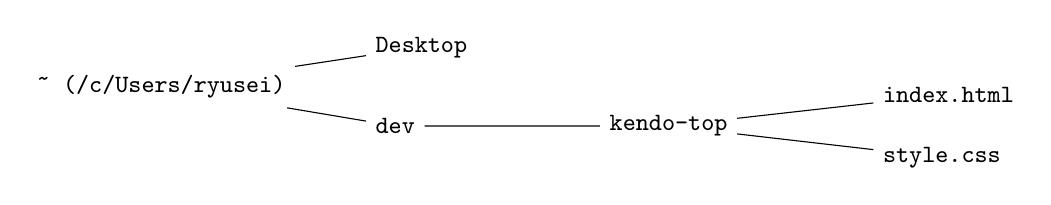
\begin{tikzpicture}[font=\ttfamily\small,grow'=right,level distance=2.6cm,
  level 1/.style={sibling distance=1cm},level 2/.style={sibling distance=0.8cm},
  every node/.style={anchor=west}]
\node {\textasciitilde\ (/c/Users/ryusei)}
  child {node {Desktop}}
  child {node {dev}
    child {node {kendo-top}
      child {node {index.html}}
      child {node {style.css}}}
  };
\end{tikzpicture}
\end{center}

\begin{itemize}
  \item \term{絶対パス}：一番上から書く住所。例：\code{/c/Users/ryusei/dev/kendo-top/index.html}
  \item \term{相対パス}：いま居る場所から見た住所。\code{dev} に居るなら \code{kendo-top/index.html}
  \item \code{.}（ドット1つ）は「いま居る場所」、\code{..}（ドット2つ）は「1つ上の階層」
\end{itemize}

\section{基本コマンド}

\begin{center}\small
\begin{tabularx}{\linewidth}{l l X}
\toprule
コマンド & 由来 & すること \\
\midrule
\code{pwd} & print working directory & いま居る場所を表示する \\
\code{ls} & list & 中にあるファイル・フォルダを一覧表示する（\code{ls -a} で隠しファイルも） \\
\code{cd 場所} & change directory & 移動する。\code{cd ..} で1つ上、\code{cd} だけでホームに戻る \\
\code{mkdir 名前} & make directory & フォルダを作る \\
\code{touch 名前} & & 空のファイルを作る \\
\code{cat ファイル} & concatenate & ファイルの中身を表示する \\
\code{cp 元 先} & copy & コピーする \\
\code{mv 元 先} & move & 移動する／名前を変える \\
\code{rm ファイル} & remove & 削除する（\textbf{ゴミ箱に入らない}） \\
\code{code .} & & いまの場所を VS Code で開く \\
\code{explorer .} & & いまの場所をエクスプローラーで開く \\
\code{clear} & & 画面をきれいにする（\key{Ctrl}+\key{L} でも同じ） \\
\bottomrule
\end{tabularx}
\end{center}

\begin{caution}[rm は取り消せない]
\code{rm} で消したファイルはゴミ箱に入らず、そのまま消えます。
特に \code{rm -rf}（フォルダごと強制削除）は、場所を間違えると大事なものまで消えます。
Claude Code が \code{rm -rf} を実行しようとしたら、\textbf{どこを消そうとしているのか必ず確かめてから}許可してください。
\end{caution}

\section{便利な操作}

\begin{center}\small
\begin{tabularx}{\linewidth}{l X}
\toprule
操作 & 効果 \\
\midrule
\key{Tab} & 名前の続きを自動で補完する。\textbf{打ち間違いが減るので積極的に使う} \\
\key{↑} \key{↓} & 前に打ったコマンドを呼び出す \\
\key{Ctrl}+\key{C} & 実行中のコマンドを止める（Git Bash ではコピーではない） \\
\key{Shift}+\key{Insert} & 貼り付け（右クリック → Paste でも可） \\
\code{q} & \code{git log} などの一覧表示から抜ける \\
\bottomrule
\end{tabularx}
\end{center}

\section{ハンズオン}

\begin{step}{作業フォルダを作る}
\sheet{4-2}
\begin{terminal}[Git Bash]
$ cd
$ pwd
/c/Users/ryusei
$ mkdir dev
$ cd dev
$ pwd
/c/Users/ryusei/dev
\end{terminal}
これで、作業フォルダ \verb|~/dev| ができました。この先の作業は、すべてこの中で行います。
\end{step}

\begin{step}{練習用のフォルダとファイルを作って動かす}
\begin{terminal}[Git Bash]
$ mkdir terminal-practice
$ cd terminal-practice
$ touch memo.txt
$ echo "面打ち 100本" > memo.txt
$ cat memo.txt
面打ち 100本
$ echo "小手面 50本" >> memo.txt
$ cat memo.txt
面打ち 100本
小手面 50本
$ cp memo.txt memo-backup.txt
$ ls
memo-backup.txt  memo.txt
$ mv memo-backup.txt old.txt
$ ls
memo.txt  old.txt
$ rm old.txt
$ ls
memo.txt
\end{terminal}
\code{>} はファイルに上書き、\code{>>} はファイルの末尾に追記、という意味です。
\end{step}

\begin{step}{VS Code とエクスプローラーで確かめる}
\begin{terminal}[Git Bash]
$ code .
$ explorer .
\end{terminal}
VS Code とエクスプローラーの両方で \code{memo.txt} が見えれば、
「ターミナルで操作したものと、マウスで見ているものは同じもの」だと確かめられたことになります。
\end{step}

\begin{challenge}{ターミナルだけで部の稽古メモを作る}
\sheet{4-3}
マウスを使わずに、次の状態を作ってください。
\begin{enumerate}
  \item \verb|~/dev/terminal-practice| の中に \code{keiko} というフォルダを作る
  \item その中に \code{monday.txt} と \code{thursday.txt} を作り、それぞれに稽古メニューを2行ずつ書く
  \item \code{thursday.txt} を \code{saturday.txt} という名前に変える
  \item \code{cat} で2つのファイルの中身を表示し、その画面をスクショしてスプシの詰まりメモ欄に「完了」と書く
\end{enumerate}
\end{challenge}

\begin{checklist}
\begin{itemize}
  \checkitem プロンプトを見て、いま居る場所を言える
  \checkitem 絶対パスと相対パスの違いを説明できる
  \checkitem \code{cd}・\code{ls}・\code{mkdir}・\code{cat} を、表を見ずに使える
  \checkitem \key{Tab} で補完できる
  \checkitem \code{rm} が危ない理由を言える
\end{itemize}
\end{checklist}

\chapter{Git と GitHub の基本}
\sheet{5-1〜5-6}

\section{Git がないと何が困るか}

レポートを書いていて、こんなファイルが並んだことはありませんか。

\begin{center}\ttfamily\small
\begin{tabular}{l}
レポート.docx\\
レポート\_修正.docx\\
レポート\_修正2.docx\\
レポート\_最終版.docx\\
レポート\_最終版\_v2\_本当に最終.docx
\end{tabular}
\end{center}

どれが最新なのか、何を変えたのか、どこで壊れたのかが分からなくなります。
これを人数分・ファイル数百個分でやるのが Web 開発です。
\term{Git}（ギット）は、ファイルを上書きしながら、\textbf{いつ・誰が・何を・なぜ変えたか}を全部記録してくれる道具です。

\section{Git の3つの場所}

Git を使うとき、ファイルは次の4つの場所を行き来します。最初はこの図だけ覚えれば十分です。

\begin{center}
\begin{tikzpicture}[font=\sffamily\small,
  area/.style={draw,rounded corners=3pt,minimum width=2.9cm,minimum height=2.3cm,align=center,fill=white},
  arr/.style={-{Stealth[length=2.5mm]},thick}]
  \node[area,draw=kincha] (w) {\textbf{作業場}\\{\scriptsize ワーキングツリー}\\[3pt]{\scriptsize いま編集している}\\{\scriptsize ファイル}};
  \node[area,draw=kon,right=1.1cm of w] (s) {\textbf{準備エリア}\\{\scriptsize ステージ}\\[3pt]{\scriptsize 次に記録する}\\{\scriptsize 予定のもの}};
  \node[area,draw=matcha,right=1.1cm of s] (r) {\textbf{記録}\\{\scriptsize ローカルリポジトリ}\\[3pt]{\scriptsize 自分の PC の}\\{\scriptsize 履歴}};
  \node[area,draw=gray,right=1.1cm of r] (g) {\textbf{GitHub}\\{\scriptsize リモートリポジトリ}\\[3pt]{\scriptsize クラウドの}\\{\scriptsize 履歴}};
  \draw[arr,kincha] (w) -- node[above,font=\ttfamily\scriptsize]{add} (s);
  \draw[arr,kon] (s) -- node[above,font=\ttfamily\scriptsize]{commit} (r);
  \draw[arr,matcha] (r) -- node[above,font=\ttfamily\scriptsize]{push} (g);
  \draw[arr,gray] (g.south) to[bend left=25] node[below,font=\ttfamily\scriptsize]{pull / clone} (w.south);
  \node[draw=gray!50,dashed,rounded corners,fit=(w)(s)(r),inner sep=6pt,label={[font=\scriptsize]above:あなたの PC（ローカル）}] {};
\end{tikzpicture}
\end{center}

\begin{description}[font=\sffamily\bfseries]
  \item[add] 「このファイルの変更を次の記録に入れる」と選ぶ
  \item[commit] 選んだ変更を、メッセージ付きで1つの記録（\term{コミット}）にする。ゲームのセーブに近い
  \item[push] 自分の PC にある記録を GitHub に送る
  \item[pull / clone] GitHub にある記録を自分の PC に持ってくる
\end{description}

\begin{why}[なぜ add と commit が分かれているのか]
1回の作業で「トップページの文言修正」と「FAQ の追加」を同時にやってしまったとします。
add で文言修正のファイルだけを選んで commit し、次に FAQ のファイルを選んで commit すれば、
\textbf{1つのコミットに1つの意味}を持たせられます。
あとで「FAQ の追加だけ取り消したい」となったときに、これが効いてきます。
\end{why}

\section{はじめてのリポジトリ}

\begin{step}{GitHub にリポジトリを作る}
\sheet{5-2}
\url{https://github.com/new} を開き、次のように入力して \btn{Create repository} を押します。
\screenshot[0.85]{github-new-repo.jpg}
\begin{itemize}
  \item \menu{Repository name}：\code{git-practice}
  \item \menu{Choose visibility}：\textbf{Public}
  \item \menu{Add README}：\textbf{Off のまま}（README は自分で作るため）
\end{itemize}
作ると、\code{…or push an existing repository from the command line} という説明が出た画面になります。
この画面は開いたままにしておきます。
\end{step}

\begin{step}{ローカルにリポジトリを作る}
\begin{terminal}[Git Bash]
$ cd ~/dev
$ mkdir git-practice
$ cd git-practice
$ git init
Initialized empty Git repository in C:/Users/ryusei/dev/git-practice/.git/
$ ls -a
.  ..  .git
\end{terminal}
\code{.git} という隠しフォルダが、Git の記録帳です。\textbf{このフォルダは手で触らないでください。}
\end{step}

\begin{step}{README を書く}
\begin{terminal}[Git Bash]
$ code README.md
\end{terminal}
VS Code が開くので、次の内容を書いて \key{Ctrl}+\key{S} で保存します。
\begin{filebox}{README.md}
\begin{Piton}[language=code]
# git-practice

Git を練習するためのリポジトリです。

## 自己紹介

- 名前：柴山りゅうせい
- 所属：理工学部 応用化学科 2年／理工体剣道部
- 好きな技：（ここに書く）
\end{Piton}
\end{filebox}
\code{.md} は \term{Markdown}（マークダウン）という書式です。
\code{\#} が見出し、\code{-} が箇条書きになります。GitHub ではきれいに整えて表示されます。
\end{step}

\begin{step}{status → add → commit}
\begin{terminal}[Git Bash]
$ git status
On branch main
No commits yet
Untracked files:
  (use "git add <file>..." to include in what will be committed)
        README.md

$ git add README.md
$ git status
Changes to be committed:
        new file:   README.md

$ git commit -m "docs: README を追加"
[main (root-commit) 3f2a1c9] docs: README を追加
 1 file changed, 9 insertions(+)
\end{terminal}
\textbf{\code{git status} は何度打ってもかまいません。}迷ったらまず \code{git status} です。
いまどの場所に何があるのかを教えてくれます。
\end{step}

\begin{step}{GitHub に push する}
さっき開いておいた GitHub の画面にある \textbf{SSH} のアドレス（\code{git@github.com:...}）を使います。
\begin{terminal}[Git Bash]
$ git remote add origin git@github.com:shibayama-ryusei/git-practice.git
$ git push -u origin main
...
To github.com:shibayama-ryusei/git-practice.git
 * [new branch]      main -> main
\end{terminal}
GitHub の画面を再読み込みして、README が表示されていれば成功です。
\code{origin} は「GitHub 側のリポジトリ」につけたあだ名です。
\code{-u} は初回だけ付ければよく、2回目からは \code{git push} だけで送れます。
\end{step}

\section{コミットメッセージの書き方}

この教材と本番のリポジトリでは、コミットメッセージを次の形で書きます（\term{Conventional Commits}）。

\begin{center}\small
\begin{tabularx}{\linewidth}{l l X}
\toprule
種類 & 使うとき & 例 \\
\midrule
\code{feat} & 新しい機能やページを足した & \code{feat: FAQ ページを追加} \\
\code{fix} & バグを直した & \code{fix: スマホで見出しがはみ出るのを修正} \\
\code{style} & 見た目だけを変えた & \code{style: ボタンの色を紺に変更} \\
\code{docs} & 説明文や README を変えた & \code{docs: README に起動方法を追記} \\
\code{refactor} & 動きは同じまま、書き方を整理した & \code{refactor: 部員表示を関数に切り出す} \\
\code{chore} & 設定などの雑務 & \code{chore: .gitignore を追加} \\
\bottomrule
\end{tabularx}
\end{center}

\begin{tip}[よいコミットの大きさ]
「1つのコミット＝説明が1行で済む変更」が目安です。
メッセージに「と」を書きたくなったら（「見出しを直したのと、FAQ を足した」）、コミットを分けるサインです。
こまめにコミットしておくと、壊したときに戻れる地点が増えます。
\end{tip}

\section{差分を見る}

\begin{step}{変更を加えて diff を見る}
README の「好きな技」を書き換えて保存してから、次を打ちます。
\begin{terminal}[Git Bash]
$ git diff
diff --git a/README.md b/README.md
@@ -7,4 +7,4 @@
 - 名前：柴山りゅうせい
 - 所属：理工学部 応用化学科 2年／理工体剣道部
-- 好きな技：（ここに書く）
+- 好きな技：出小手
\end{terminal}
\code{-} で始まる行が消えた行、\code{+} で始まる行が足された行です。
\textbf{\code{git diff} を読む力は、AI と開発するときに一番大事な力です。}
Claude Code が何を変えたのかは、最終的にはこれで確かめます。
\end{step}

\begin{step}{履歴を見る}
変更を add・commit・push してから、履歴を見ます。
\begin{terminal}[Git Bash]
$ git add README.md
$ git commit -m "docs: 好きな技を追記"
$ git push
$ git log --oneline
a81d0e4 (HEAD -> main, origin/main) docs: 好きな技を追記
3f2a1c9 docs: README を追加
\end{terminal}
\end{step}

\begin{tip}[VS Code でも差分は見られる]
VS Code の左端にある、枝分かれしたアイコン（ソース管理）を押すと、変更したファイルの一覧が出ます。
ファイル名を押すと、変更前と変更後が左右に並んで表示されます。
ターミナルの \code{git diff} と同じものなので、見やすい方を使ってかまいません。
\end{tip}

\section{取り消し方}

\begin{center}\small
\begin{tabularx}{\linewidth}{X l}
\toprule
状況 & コマンド \\
\midrule
保存したけど、まだ add していない変更をなかったことにしたい & \code{git restore ファイル名} \\
add したけど、やっぱり準備エリアから外したい & \code{git restore --staged ファイル名} \\
直前のコミットのメッセージを直したい（\textbf{push する前だけ}） & \code{git commit --amend -m "新しいメッセージ"} \\
\bottomrule
\end{tabularx}
\end{center}

\begin{caution}[push した後の履歴は書き換えない]
\code{--amend} や \code{git reset} で履歴を書き換えたあとに push しようとすると、拒否されます。
そこで \code{git push -f}（強制 push）を使うと、GitHub 側の履歴を上書きしてしまい、
チーム開発では他の人の作業を消す事故になります。
\textbf{強制 push は、三角に相談してからでないと使わない}と決めておいてください。
\end{caution}

\section{.gitignore：Git に記録させないもの}

パスワードや、自動で作られる大量のファイルは、Git に記録してはいけません。
記録させないファイルを書いておくのが \code{.gitignore} です。

\begin{filebox}{.gitignore（第2巻以降で使う例）}
\begin{Piton}[language=code]
# 自動で作られる大量のファイル
node_modules/
.next/

# 秘密の設定（API キーなど）
.env*
!.env.example

# OS が勝手に作るファイル
Thumbs.db
.DS_Store
\end{Piton}
\end{filebox}

\begin{caution}[秘密情報を push してしまったら]
API キーやパスワードを含むファイルを GitHub に push してしまったら、\textbf{すぐに三角に連絡してください}。
コミットを消しても、一度公開されたキーは誰かに見られた前提で扱う必要があり、キーそのものを作り直す必要があります。
隠さずにすぐ言ってくれれば、被害はほぼ防げます。
\end{caution}

\section{よくあるエラー}

\begin{center}\small
\begin{tabularx}{\linewidth}{>{\ttfamily\raggedright\arraybackslash}p{5.2cm} X}
\toprule
\normalfont エラーの一部 & 原因と対処 \\
\midrule
Permission denied (publickey) & SSH 鍵が GitHub に登録されていないか、HTTPS のアドレスと混ざっている。\code{ssh -T git@github.com} で確かめる \\
\addlinespace
Please tell me who you are & 初期設定（\code{user.name}、\code{user.email}）をしていない。第3章に戻る \\
\addlinespace
nothing to commit, working tree clean & 記録する変更がない。保存（\key{Ctrl}+\key{S}）し忘れていないか確認する \\
\addlinespace
! [rejected] ... (fetch first) & GitHub 側に、自分の PC にない記録がある。\code{git pull} してから push する \\
\addlinespace
not a git repository & Git の管理下にないフォルダにいる。\code{pwd} で場所を確認する \\
\addlinespace
\normalfont（\code{-m} を付け忘れて VS Code のタブが開いた） & メッセージ入力用のタブ。1行目にメッセージを書いて保存し、タブを閉じれば commit される \\
\bottomrule
\end{tabularx}
\end{center}

\begin{challenge}{わざと失敗して、元に戻す}
\sheet{5-6}
\code{git-practice} で次のことを順にやり、各段階で \code{git status} の表示がどう変わるかをメモしてください。
\begin{enumerate}
  \item README を適当に書き換えて保存する → \code{git restore} で元に戻す
  \item \code{keiko.md} という新しいファイルを作り、add する → \code{git restore --staged} で準備エリアから外す
  \item \code{keiko.md} を commit する。そのときメッセージをわざと間違える → \code{--amend} で直してから push する
\end{enumerate}
「どの場所にあるファイルを、どの場所に戻したのか」を、本章の3つの場所の図を使って定例で説明します。
\end{challenge}

\begin{checklist}
\begin{itemize}
  \checkitem 作業場・準備エリア・ローカルの記録・GitHub の4つの関係を図で説明できる
  \checkitem \code{status → add → commit → push} を、資料を見ずにできる
  \checkitem \code{git diff} の \code{+} と \code{-} を読める
  \checkitem Conventional Commits の形でメッセージを書ける
  \checkitem 強制 push をしてはいけない理由を言える
  \checkitem 秘密情報を push してしまったときの対応を言える
\end{itemize}
\end{checklist}

\chapter{Claude Code と組む}
\sheet{6-1〜6-5}

\section{Claude Code とは}

\term{Claude Code} は、ターミナルの中で動く AI です。チャットの Claude と違うのは、次の2点です。

\begin{itemize}
  \item \textbf{あなたの PC のファイルを読んで、書き換えられる}
  \item \textbf{コマンドを実行できる}（\code{git status} や \code{npm run dev} など）
\end{itemize}

つまり、「このフォルダのコードを読んで、ここを直して」と頼むと、本当に直してくれます。
強力な分、\textbf{何をさせたのかを自分で把握しておく}ことが大事になります。

\section{起動と終了}

\begin{step}{練習用リポジトリで起動する}
\begin{terminal}[Git Bash]
$ cd ~/dev/git-practice
$ claude
\end{terminal}
\textbf{Claude Code は、起動した場所のフォルダを「作業場所」として扱います。}
必ず作業したいリポジトリに \code{cd} してから起動してください。
ホームフォルダ（\code{\textasciitilde}）で起動すると、PC 中のファイルが対象になってしまいます。
\end{step}

最初に「このフォルダを信頼しますか」と聞かれたら、自分のリポジトリであることを確かめてから \code{Yes} を選びます。

\begin{center}\small
\begin{tabularx}{\linewidth}{l X}
\toprule
入力 & 効果 \\
\midrule
普通の文章 & Claude への依頼 \\
\code{/exit} & 終了する \\
\code{/clear} & 会話をリセットする（\textbf{別の作業に移るときは必ず}） \\
\code{/compact} & これまでの会話を要約して軽くする \\
\code{/status} & ログイン状態や残りの使用量を見る \\
\code{/help} & コマンドの一覧 \\
\key{Esc} & Claude の作業を途中で止める \\
\key{Esc} を2回 & 前の発言に戻ってやり直す \\
\key{Shift}+\key{Tab} & 動作モードを切り替える（下で説明） \\
\bottomrule
\end{tabularx}
\end{center}

\section{許可を求められたら}

Claude Code はファイルを書き換える前や、コマンドを実行する前に、許可を求めてきます。

\begin{wintermwin}[0.9\linewidth]{MINGW64:/c/Users/ryusei/dev/git-practice}
Bash command\\[2pt]
\hspace*{1em}git add README.md \&\& git commit -m "docs: 自己紹介を更新"\\[4pt]
Do you want to proceed?\\
{\color{kincha!80!white}> 1. Yes}\\
\hspace*{0.75em}2. Yes, and don't ask again for git commit commands\\
\hspace*{0.75em}3. No, and tell Claude what to do differently (esc)
\end{wintermwin}

\begin{caution}[許可する前に読む]
\begin{itemize}
  \item \textbf{何をしようとしているか分からないコマンドは、許可しない。}3（No）を選び、「このコマンドは何をするものか説明して」と聞く
  \item \code{rm -rf}、\code{git push -f}、\code{git reset --hard} が出てきたら、必ず止まって確認する
  \item 「2. 今後は聞かない」は、\code{git status} のような\textbf{読むだけのコマンド}にだけ使う
\end{itemize}
\end{caution}

\key{Shift}+\key{Tab} で切り替えられる主なモードは、次の通りです。

\begin{center}\small
\begin{tabularx}{\linewidth}{l X l}
\toprule
モード & 動き & この教材での使い方 \\
\midrule
通常 & 書き換えのたびに許可を求める & \textbf{基本はこれ} \\
plan mode & 書き換えずに、計画だけ立てる & 大きめの作業の前に、方針を相談するとき \\
accept edits & ファイルの書き換えは許可なしで進める & 第2巻以降、慣れてから \\
\bottomrule
\end{tabularx}
\end{center}

\section{CLAUDE.md：Claude への申し送り}

リポジトリの一番上に \code{CLAUDE.md} というファイルを置くと、Claude Code は起動するたびにそれを読みます。
「このプロジェクトはこういうルールで作っている」という申し送り帳です。

\begin{filebox}{CLAUDE.md（例：練習用リポジトリに置いてあるもの）}
\begin{Verbatim}[fontsize=\small]
# このリポジトリについて
理工体剣道部サイトの練習版。作っているのは未経験から学習中の柴山。

## Claude へのお願い
- 答えのコードをいきなり全部書かず、まず方針と理由を説明する
- 新しい用語が出てきたら、1行で意味を添える
- 変更したら、どのファイルの何行目を、なぜ変えたかを最後にまとめる
- git push、ファイルの削除、強制系のコマンドは実行前に必ず確認する
\end{Verbatim}
\end{filebox}

練習用リポジトリには、先輩がこれを用意してあります。
本番の \code{rikotaikendo-web} にも \code{CLAUDE.md} があり、技術構成やルールが書いてあります。
第5巻で読みます。

\begin{step}{練習用リポジトリを clone して、CLAUDE.md を読む}
\sheet{6-3}
GitHub にあるリポジトリを丸ごと手元にコピーすることを \term{clone}（クローン）といいます。
\begin{terminal}[Git Bash]
$ cd ~/dev
$ git clone git@github.com:yutomi141/rikotaikendo-practice.git
$ cd rikotaikendo-practice
$ ls
CLAUDE.md  README.md  docs
$ cat CLAUDE.md
\end{terminal}
\code{CLAUDE.md} を読んで、Claude がこのリポジトリでどう振る舞うよう頼まれているかを確かめてください。
次に、ここで Claude Code を起動して、教材について質問してみます。
\begin{prompt}
docs/textbook/vol1/chapters/ch05-git.tex を読んで、git add と git commit が分かれている理由を、剣道の稽古にたとえて説明して。
\end{prompt}
\textbf{このリポジトリの \code{main} には、直接 push できない設定になっています。}
変更を加えるのは第2巻からで、そのときはブランチを切って PR を出します。
教材が更新されたら、このフォルダで \code{git pull} すると最新になります。
\end{step}

\section{頼み方の5原則}

\begin{enumerate}
  \item \textbf{目的を書く}：何のためにやるのか（「新入生がスマホで見るので」）
  \item \textbf{範囲を書く}：触ってよいファイル、触ってはいけないファイル
  \item \textbf{完成の条件を書く}：どうなったら終わりか（「幅375pxで横にはみ出ない」）
  \item \textbf{小さく頼む}：1回の依頼で1つのこと
  \item \textbf{理由を聞く}：「なぜそうしたのか」まで答えてもらう
\end{enumerate}

\begin{badprompt}
いい感じのトップページを作って
\end{badprompt}

\begin{prompt}
index.html のヒーロー部分（\verb|<section class="hero">|）だけを直したい。\\
目的：新入生がスマホで開いたとき、部の名前と「稽古見学歓迎」がすぐ目に入るようにしたい。\\
範囲：index.html と style.css のヒーロー部分だけ。ほかのセクションは触らないで。\\
完成の条件：幅 375px の画面で、文字が画像からはみ出さないこと。\\
コードを書く前に、どう直すつもりかと、その理由を先に説明して。
\end{prompt}

\section{育てるサイクル}

AI との開発は、次のサイクルの繰り返しです。

\begin{center}
\begin{tikzpicture}[font=\sffamily\small,
  st/.style={draw=kon,circle,minimum size=2.3cm,align=center,fill=white,text width=2cm},
  arr/.style={-{Stealth[length=2.5mm]},very thick,kon!60}]
  \node[st] (a) at (90:2.6) {① 頼む\\{\scriptsize 小さく・具体的に}};
  \node[st] (b) at (0:2.6) {② 差分を読む\\{\scriptsize \texttt{git diff}}};
  \node[st] (c) at (-90:2.6) {③ 確かめる\\{\scriptsize ブラウザで見る}};
  \node[st] (d) at (180:2.6) {④ commit\\{\scriptsize 1つの意味で}};
  \draw[arr] (a) to[bend left=20] (b); \draw[arr] (b) to[bend left=20] (c);
  \draw[arr] (c) to[bend left=20] (d); \draw[arr] (d) to[bend left=20] (a);
\end{tikzpicture}
\end{center}

\textbf{②と③を飛ばさない}ことが一番大事です。
Claude は「できました」と言いますが、本当にできているかは、あなたが差分を読み、画面で確かめるまで分かりません。
③でおかしかったら、commit せずに①に戻ります。
うまくいったら④でセーブし、次の小さな依頼に進みます。

\section{「教えてもらう」使い方}

Claude Code は、作業させるだけでなく、先生としても使えます。

\begin{prompt}[分からないことを聞く]
いま git diff で出た「@@ -7,4 +7,4 @@」は何を意味している？ 1つずつ説明して。
\end{prompt}

\begin{prompt}[自分の理解を確かめる]
CSS の position: absolute について、私はこう理解している：「親の要素を基準に、好きな位置に置ける」。\\
この理解で合っている？ 足りない点や間違いがあれば、例を使って教えて。
\end{prompt}

\begin{prompt}[エラーを読む練習]
このエラーの原因を教えて。ただし、直し方はまだ言わないで。私が先に直し方を考えるから、そのあと答え合わせして。\\
（エラーメッセージを全文貼る）
\end{prompt}

\section{使用量を節約する}

Pro の使用量は、Claude が読んだり書いたりする量に比例して減ります。

\begin{itemize}
  \item \textbf{作業が変わったら \code{/clear}}：前の作業の会話を引きずると、毎回それを読み直すので減りが早くなる
  \item \textbf{範囲を絞る}：「このファイルの、この部分」と指定すると、余計なファイルを読まずに済む
  \item \textbf{大きい作業は plan mode で方針を決めてから}：やり直しが減る
  \item \textbf{簡単なことは自分でやる}：1文字の修正や \code{git status} を Claude に頼まない
  \item \code{/status} で残量を確認する習慣をつける
\end{itemize}

\begin{tip}[上限に達した日にできること]
上限に達しても、学習は止まりません。次のことを進めてください。
\begin{itemize}
  \item 教材を先に読み進める
  \item 自分で書いたコード、Claude が書いたコードを読み直し、分からない行に印をつけておく（次に聞く）
  \item 小さな修正を自分の手でやってみる
  \item 腕だめしの「どこを、どう変えればよいか」のメモを先に書いておく
\end{itemize}
\end{tip}

\section{AI と付き合う3つの掟}

\begin{tcolorbox}[kwbase,colback=kon!4,colframe=kon,title={3つの掟}]
\begin{enumerate}
  \item \textbf{説明できないコードは、commit しない。}分からない行があれば、分かるまで聞く。
  \item \textbf{秘密は渡さない。}秘密鍵、パスワード、本番の API キーは、Claude にも見せない。
  \item \textbf{AI の「できました」を信じない。自分の目で確かめる。}
\end{enumerate}
\end{tcolorbox}

\begin{step}{Claude Code で README を育てる}
\sheet{6-5}
\code{git-practice} で Claude Code を起動し、次のことを頼んでみましょう。
\begin{enumerate}
  \item 「README.md に『剣道部での役割』という見出しを足して、箇条書きで3つ書けるように枠だけ作って。中身は私が書く」
  \item 許可を求められたら、内容を読んでから許可する
  \item \code{/exit} で終了し、\code{git diff} で何が変わったかを自分で確認する
  \item 中身を自分で書き、commit して push する
\end{enumerate}
\end{step}

\begin{checklist}
\begin{itemize}
  \checkitem 作業したいリポジトリに \code{cd} してから Claude Code を起動している
  \checkitem 許可を求められたとき、コマンドの意味を確かめてから選べる
  \checkitem 頼み方の5原則に沿って依頼を書ける
  \checkitem 育てるサイクル（頼む→差分→確かめる→commit）を回せる
  \checkitem \code{/clear} を使う場面を言える
  \checkitem 3つの掟を言える
\end{itemize}
\end{checklist}

\chapter{フェーズ① HTML と CSS で部のトップページをつくる}
\sheet{7-1〜7-10}

いよいよ Web ページを作ります。完成形は次のページです。
PC で見たとき（左）と、スマホで見たとき（右）で、レイアウトが変わります。

\begin{center}
\fcolorbox{gray!50}{white}{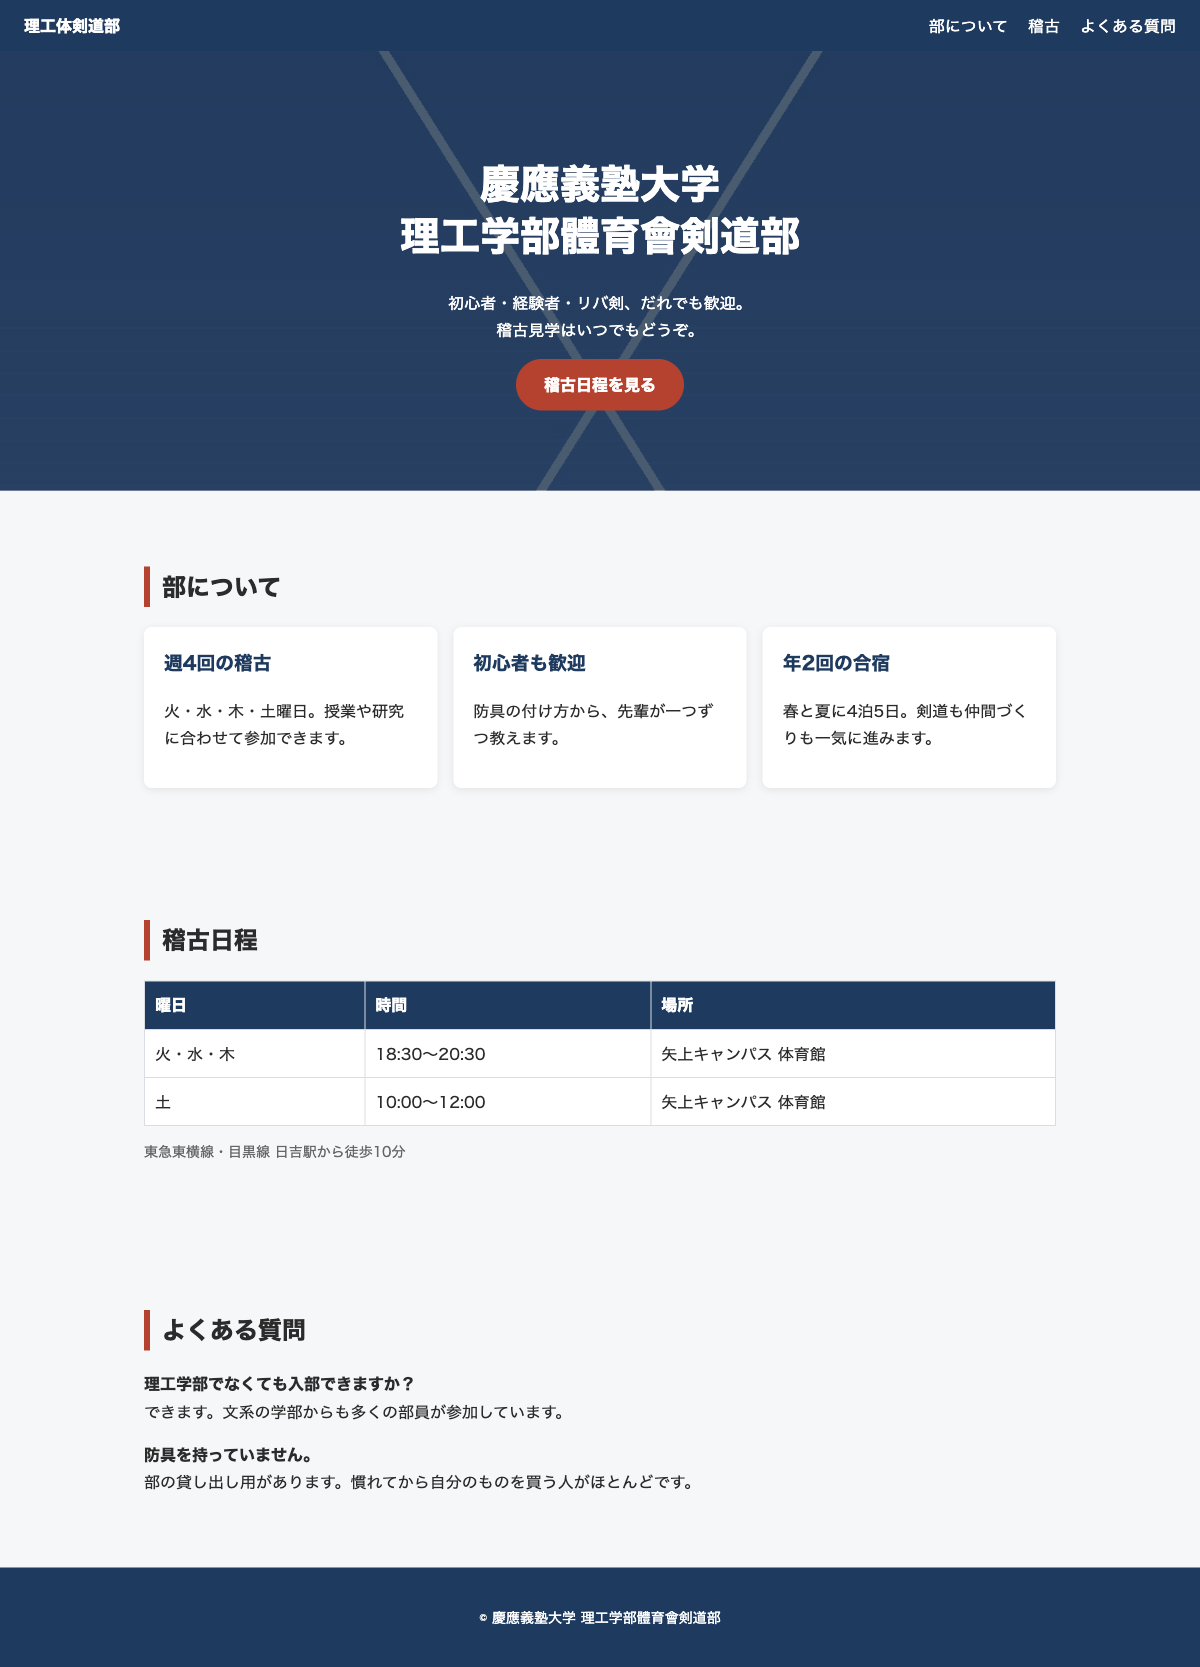
\includegraphics[width=0.58\linewidth]{kendo-top-pc.png}}\hspace{6mm}
\fcolorbox{gray!50}{white}{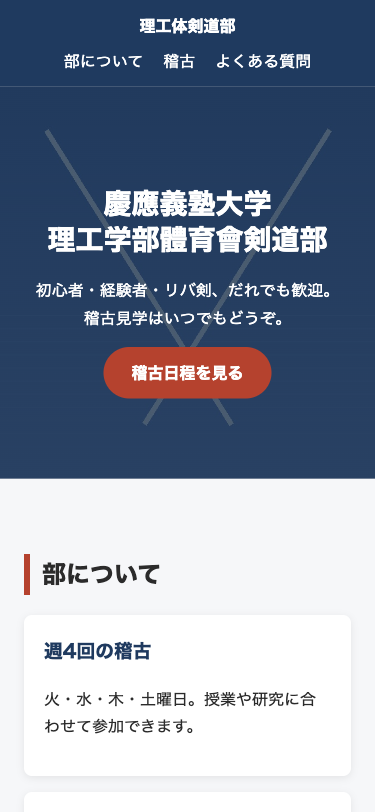
\includegraphics[width=0.25\linewidth]{kendo-top-sp.png}}
\end{center}
\figcap{完成イメージ（左：PC　右：スマホ）}

\begin{tip}[この章の進め方]
この章のコードは、\textbf{Claude に書かせず、自分の手で打ってください}。
HTML と CSS は、これから先ずっと読み書きする言葉です。一度自分の手で打っておくと、
第2巻以降で Claude が書いたコードを読むときの速さが全く違います。
打ち間違いでうまく表示されないときに原因を探すのも、大事な練習です。
\end{tip}

\section{準備：リポジトリを作る}

\begin{step}{kendo-top リポジトリを作る}
\sheet{7-1}
\begin{enumerate}
  \item GitHub で \code{kendo-top} という名前の Public リポジトリを作ります（README は Off）。
  \item 手元にフォルダを作り、Git の管理を始めます。
\end{enumerate}
\begin{terminal}[Git Bash]
$ cd ~/dev
$ mkdir kendo-top
$ cd kendo-top
$ git init
$ mkdir images
$ touch index.html style.css
$ git remote add origin git@github.com:shibayama-ryusei/kendo-top.git
$ code .
\end{terminal}
\end{step}

\begin{step}{トップ画像を用意する}
部の集合写真を三角からもらい、\code{images/hero.jpg} という名前で保存します。
\end{step}

\begin{caution}[ネットに載せてよい写真か]
このリポジトリは Public（誰でも見られる）で、GitHub Pages で公開もします。
\textbf{部員の顔が写った写真を使うときは、公開してよいものか三角に確認してください。}
本番のサイトでも、写真や名前の扱いには同じ注意が必要です。
\end{caution}

\section{HTML の骨組み}

\term{HTML} は、\term{タグ}と呼ばれる \code{<名前>} の印で文章を挟み、「ここは見出し」「ここは段落」と意味を付けていく言葉です。

\begin{center}
\begin{tikzpicture}[font=\ttfamily\small]
  \node[fill=kon!10,inner sep=3pt] (o) {<h1>};
  \node[right=0pt of o,inner sep=3pt] (t) {理工学部體育會剣道部};
  \node[right=0pt of t,fill=kon!10,inner sep=3pt] (c) {</h1>};
  \draw[<-,gray] (o.south) -- ++(0,-0.5) node[below,font=\sffamily\scriptsize]{開始タグ};
  \draw[<-,gray] (t.south) -- ++(0,-0.5) node[below,font=\sffamily\scriptsize]{中身};
  \draw[<-,gray] (c.south) -- ++(0,-0.5) node[below,font=\sffamily\scriptsize]{終了タグ（/ が付く）};
\end{tikzpicture}
\end{center}

\begin{step}{骨組みを書く}
\sheet{7-2}
\code{index.html} に次のように書きます。
\begin{filebox}{index.html}
\begin{Piton}[language=code]
<!DOCTYPE html>
<html lang="ja">
<head>
  <meta charset="UTF-8">
  <meta name="viewport" content="width=device-width, initial-scale=1.0">
  <title>慶應義塾大学 理工学部體育會剣道部</title>
  <link rel="stylesheet" href="style.css">
</head>
<body>
  <!-- ここにページの中身を書いていく -->
</body>
</html>
\end{Piton}
\end{filebox}

\begin{description}[font=\ttfamily\bfseries,style=nextline,leftmargin=2em]
  \item[<head>] ページの「設定」を書く場所。画面には表示されない
  \item[<meta charset="UTF-8">] 文字化けを防ぐおまじない。日本語を使うなら必須
  \item[<meta name="viewport" ...>] スマホで正しい幅で表示させる設定。\textbf{これがないとスマホで文字が極小になる}
  \item[<title>] ブラウザのタブに出る名前。Google の検索結果にも出る
  \item[<link rel="stylesheet" ...>] 見た目を決める CSS ファイルを読み込む
  \item[<body>] 画面に表示される中身を書く場所
  \item[<!-- -->] コメント。ブラウザは無視する。メモに使う
\end{description}
\end{step}

\section{ページを表示して確かめる}

\begin{step}{ローカルでページを開く}
\sheet{7-3}
VS Code のターミナル（\key{Ctrl}+\key{@}）で、次のように打ちます。
\begin{terminal}[Git Bash]
$ npx serve .
Need to install the following packages:
serve@14.x.x
Ok to proceed? (y) y

   ┌────────────────────────────────────────┐
   │   Serving!                             │
   │   - Local:    http://localhost:3000    │
   └────────────────────────────────────────┘
\end{terminal}
ブラウザで \url{http://localhost:3000} を開きます。真っ白なページで、タブに部の名前が出ていれば成功です。
止めるときは、ターミナルで \key{Ctrl}+\key{C} を押します。
\end{step}

\begin{why}[localhost とは]
\code{localhost} は「自分の PC」を指す特別な名前です。
\code{npx serve} は、自分の PC を小さなサーバーにして、第1章の図の「サーバー」の役をさせています。
\code{:3000} は\term{ポート番号}で、PC の中の「何番窓口か」を表します。
第2巻でサーバーの仕組みを作るときも、同じように \code{localhost} で確かめながら作ります。
\end{why}

\section{中身を書く}

\begin{step}{ヘッダーとヒーロー}
\sheet{7-4}
\code{<body>} の中のコメントを消して、次のように書きます。
\begin{filebox}{index.html（<body> の中）}
\begin{Piton}[language=code]
  <header class="site-header">
    <p class="logo">理工体剣道部</p>
    <nav>
      <ul class="nav-list">
        <li><a href="#about">部について</a></li>
        <li><a href="#practice">稽古</a></li>
        <li><a href="#faq">よくある質問</a></li>
      </ul>
    </nav>
  </header>

  <main>
    <section class="hero">
      <h1>慶應義塾大学<br>理工学部體育會剣道部</h1>
      <p>初心者・経験者・リバ剣、だれでも歓迎。<br>稽古見学はいつでもどうぞ。</p>
      <a class="button" href="#practice">稽古日程を見る</a>
    </section>

    <!-- 次の STEP で、ここにセクションを足していく -->
  </main>

  <footer class="site-footer">
    <p>&copy; 慶應義塾大学 理工学部體育會剣道部</p>
  </footer>
\end{Piton}
\end{filebox}
\end{step}

\begin{center}\small
\begin{tabularx}{\linewidth}{>{\ttfamily}l X}
\toprule
\normalfont タグ & 意味 \\
\midrule
header / main / footer & ページの頭・本体・足。意味のまとまりを示す \\
nav & サイト内の移動用メニュー \\
section & 1つの話題のまとまり \\
h1〜h6 & 見出し。数字が小さいほど大きな見出し。\textbf{h1 はページに1つ} \\
p & 段落 \\
ul / li & 箇条書きの全体／1項目 \\
a & リンク。\code{href} に行き先を書く。\code{\#about} は同じページの \code{id="about"} へ飛ぶ \\
br & 改行（終了タグなし） \\
\bottomrule
\end{tabularx}
\end{center}

\code{class="..."} は、CSS で見た目を付けるときの「名札」です。次の節で使います。

\begin{step}{部の紹介・稽古日程・よくある質問}
\sheet{7-5}
\code{<main>} の中の「次の STEP で…」のコメントを、次の3つのセクションに置き換えます。
\begin{filebox}{index.html（<main> の中、hero の下）}
\begin{Piton}[language=code]
    <section id="about" class="section">
      <h2>部について</h2>
      <div class="cards">
        <article class="card">
          <h3>週4回の稽古</h3>
          <p>火・水・木・土曜日。授業や研究に合わせて参加できます。</p>
        </article>
        <article class="card">
          <h3>初心者も歓迎</h3>
          <p>防具の付け方から、先輩が一つずつ教えます。</p>
        </article>
        <article class="card">
          <h3>年2回の合宿</h3>
          <p>春と夏に4泊5日。剣道も仲間づくりも一気に進みます。</p>
        </article>
      </div>
    </section>

    <section id="practice" class="section">
      <h2>稽古日程</h2>
      <table class="schedule">
        <tr><th>曜日</th><th>時間</th><th>場所</th></tr>
        <tr><td>火・水・木</td><td>18:30〜20:30</td><td>矢上キャンパス 体育館</td></tr>
        <tr><td>土</td><td>10:00〜12:00</td><td>矢上キャンパス 体育館</td></tr>
      </table>
      <p class="note">東急東横線・目黒線 日吉駅から徒歩10分</p>
    </section>

    <section id="faq" class="section">
      <h2>よくある質問</h2>
      <dl class="faq">
        <dt>理工学部でなくても入部できますか？</dt>
        <dd>できます。文系の学部からも多くの部員が参加しています。</dd>
        <dt>防具を持っていません。</dt>
        <dd>部の貸し出し用があります。慣れてから自分のものを買う人がほとんどです。</dd>
      </dl>
    </section>
\end{Piton}
\end{filebox}
\textbf{稽古の時間は例です。}実際の時間に書き換えてください。
\end{step}

\begin{tip}[表とリストのタグ]
\code{table}（表全体）、\code{tr}（1行）、\code{th}（見出しのマス）、\code{td}（普通のマス）。
\code{dl}・\code{dt}・\code{dd} は「用語と説明」の組で、質問と答えの組み合わせにぴったりです。
\end{tip}

ブラウザを再読み込み（\key{F5}）すると、文字だけの地味なページが表示されます。
ここまでで、一度コミットしておきましょう。

\begin{terminal}[Git Bash]
$ git add index.html images/hero.jpg
$ git commit -m "feat: トップページの HTML を作成"
\end{terminal}

\section{CSS で見た目を整える}

\term{CSS} は「どの要素に」「何を」「どうするか」を書く言葉です。

\begin{center}
\begin{tikzpicture}[font=\ttfamily\small]
  \node[fill=kon!10,inner sep=3pt] (sel) {.card};
  \node[right=2pt of sel] (b1) {\{};
  \node[right=2pt of b1,fill=kincha!15,inner sep=3pt] (prop) {color};
  \node[right=0pt of prop] (c) {:};
  \node[right=2pt of c,fill=matcha!15,inner sep=3pt] (val) {white};
  \node[right=0pt of val] (b2) {; \}};
  \draw[<-,gray] (sel.south) -- ++(0,-0.5) node[below,font=\sffamily\scriptsize,align=center]{セレクタ\\どの要素に};
  \draw[<-,gray] (prop.south) -- ++(0,-0.5) node[below,font=\sffamily\scriptsize,align=center]{プロパティ\\何を};
  \draw[<-,gray] (val.south) -- ++(0,-0.5) node[below,font=\sffamily\scriptsize,align=center]{値\\どうする};
\end{tikzpicture}
\end{center}

セレクタの書き方は、\code{.名前} で class、\code{\#名前} で id、\code{h2} のようにタグ名だけで「そのタグすべて」を指します。
\code{.section h2} のように空白で区切ると、「\code{.section} の中にある \code{h2}」という意味になります。

\begin{step}{色の約束と全体の設定}
\sheet{7-6}
\begin{filebox}{style.css}
\begin{Piton}[language=code]
/* 色の約束：ここを変えればサイト全体の色が変わる */
:root {
  --color-kon: #1f3a5f;
  --color-shu: #b5422e;
  --color-bg: #f6f7f9;
  --color-text: #2b2b2b;
}

* {
  box-sizing: border-box;
}

body {
  margin: 0;
  font-family: "Hiragino Sans", "Yu Gothic", sans-serif;
  color: var(--color-text);
  background-color: var(--color-bg);
  line-height: 1.7;
}
\end{Piton}
\end{filebox}
\code{--color-kon} は\term{CSS 変数}です。色を1か所にまとめておき、\code{var(--color-kon)} で呼び出します。
本番のサイトも、色はこうして1か所で管理しています。
\code{\#1f3a5f} は色を16進数で表したもので、赤・緑・青の強さを2桁ずつ書いています。
\end{step}

\begin{step}{ヘッダーとヒーロー}
\begin{filebox}{style.css（続き）}
\begin{Piton}[language=code]
/* ヘッダー */
.site-header {
  display: flex;
  justify-content: space-between;
  align-items: center;
  padding: 12px 24px;
  background-color: var(--color-kon);
  color: white;
}

.logo {
  margin: 0;
  font-weight: bold;
}

.nav-list {
  display: flex;
  gap: 20px;
  margin: 0;
  padding: 0;
  list-style: none;
}

.nav-list a {
  color: white;
  text-decoration: none;
}

/* ヒーロー（一番上の大きな部分） */
.hero {
  padding: 80px 24px;
  text-align: center;
  color: white;
  background: linear-gradient(rgba(31, 58, 95, 0.75), rgba(31, 58, 95, 0.75)),
    url("images/hero.jpg") center / cover;
}

.hero h1 {
  font-size: 40px;
  line-height: 1.3;
}

.button {
  display: inline-block;
  padding: 12px 28px;
  border-radius: 999px;
  background-color: var(--color-shu);
  color: white;
  text-decoration: none;
  font-weight: bold;
}
\end{Piton}
\end{filebox}
\end{step}

\section{箱の考え方：ボックスモデル}

CSS では、すべての要素を「箱」として扱います。箱は内側から順に、次の4層でできています。

\begin{center}
\begin{tikzpicture}[font=\sffamily\small]
  \draw[fill=kincha!12,draw=kincha] (0,0) rectangle (8,4.4);
  \node[anchor=north west,font=\scriptsize] at (0.1,4.35) {margin（外側の余白：となりの箱との距離）};
  \draw[fill=sumi!80,draw=sumi] (0.6,0.5) rectangle (7.4,3.8);
  \node[anchor=north west,font=\scriptsize,text=white] at (0.65,3.78) {border（枠線）};
  \draw[fill=matcha!15,draw=matcha] (0.8,0.7) rectangle (7.2,3.4);
  \node[anchor=north west,font=\scriptsize] at (0.85,3.38) {padding（内側の余白）};
  \draw[fill=white,draw=kon] (1.6,1.2) rectangle (6.4,2.8);
  \node at (4,2) {content（中身：文字や画像）};
\end{tikzpicture}
\end{center}

\code{padding: 12px 24px;} は「上下 12px、左右 24px の内側の余白」という意味です。
最初に書いた \code{box-sizing: border-box;} は、「幅を指定したら、padding と枠線もその幅の中に含める」という設定です。
これがないと、余白を足すたびに箱がはみ出していきます。

\section{横に並べる：Flexbox}

\code{display: flex;} を指定すると、その箱の\textbf{子どもたちが横一列に並びます}。
ヘッダーでロゴとメニューが左右に分かれているのは、これを使っているからです。

\begin{center}
\begin{tikzpicture}[font=\sffamily\scriptsize]
  \draw[kon,thick,rounded corners] (0,0) rectangle (9,1.2);
  \node[anchor=north west,text=kon] at (0,1.55) {\texttt{.site-header \{ display: flex; justify-content: space-between; \}}};
  \node[draw,fill=white,minimum width=2cm,minimum height=0.7cm] at (1.3,0.6) {.logo};
  \node[draw,fill=white,minimum width=3.2cm,minimum height=0.7cm] at (7.2,0.6) {nav};
  \draw[<->,shu] (2.4,0.6) -- node[above]{space-between：両端に寄せる} (5.5,0.6);
\end{tikzpicture}
\end{center}

\begin{center}\small
\begin{tabularx}{\linewidth}{>{\ttfamily}l X}
\toprule
\normalfont プロパティ & 意味 \\
\midrule
justify-content & 並ぶ方向（横）の寄せ方。\code{space-between} で両端、\code{center} で中央 \\
align-items & 並ぶ方向と直角（縦）の揃え方。\code{center} で上下中央 \\
gap & 子ども同士の間隔 \\
flex-direction & 並ぶ向き。\code{column} にすると縦に並ぶ \\
flex: 1 & （子ども側に書く）余った幅を均等に分け合う \\
\bottomrule
\end{tabularx}
\end{center}

\begin{step}{セクション・カード・表・フッター}
\sheet{7-7}
\begin{filebox}{style.css（続き）}
\begin{Piton}[language=code]
/* 各セクション共通 */
.section {
  max-width: 960px;
  margin: 0 auto;
  padding: 56px 24px;
}

.section h2 {
  border-left: 6px solid var(--color-shu);
  padding-left: 12px;
}

/* カードを横に並べる */
.cards {
  display: flex;
  gap: 16px;
}

.card {
  flex: 1;
  padding: 20px;
  background-color: white;
  border-radius: 8px;
  box-shadow: 0 2px 8px rgba(0, 0, 0, 0.08);
}

.card h3 {
  margin-top: 0;
  color: var(--color-kon);
}

/* 稽古日程の表 */
.schedule {
  width: 100%;
  border-collapse: collapse;
  background-color: white;
}

.schedule th,
.schedule td {
  padding: 10px;
  border: 1px solid #d9dde3;
  text-align: left;
}

.schedule th {
  background-color: var(--color-kon);
  color: white;
}

.note {
  font-size: 14px;
  color: #666;
}

/* よくある質問 */
.faq dt {
  font-weight: bold;
  margin-top: 16px;
}

.faq dd {
  margin-left: 0;
}

.site-footer {
  padding: 24px;
  text-align: center;
  background-color: var(--color-kon);
  color: white;
  font-size: 14px;
}
\end{Piton}
\end{filebox}
\code{max-width: 960px; margin: 0 auto;} は、「広い画面でも幅は 960px まで。左右の余白は自動で同じにする（＝中央寄せ）」という定番の書き方です。
\end{step}

\section{スマホに対応する：レスポンシブ}

このままスマホで見ると、カード3枚が横に並んだまま押しつぶされます。
画面の幅によって CSS を切り替えるのが\term{メディアクエリ}です。

\begin{step}{スマホ用の CSS を足す}
\sheet{7-8}
\begin{filebox}{style.css（一番最後に足す）}
\begin{Piton}[language=code]
/* 画面の幅が 640px 以下（スマホ）のときだけ効く */
@media (max-width: 640px) {
  .site-header {
    flex-direction: column;
    gap: 8px;
  }

  .hero h1 {
    font-size: 28px;
  }

  .cards {
    flex-direction: column;
  }
}
\end{Piton}
\end{filebox}
\end{step}

\begin{tip}[新入生はスマホで見る]
部のサイトに来る新入生のほとんどは、スマホで見ています。
作ったら\textbf{必ずスマホの幅で確かめる}ことを習慣にしてください。確かめ方は次の節で説明します。
\end{tip}

\section{開発者ツール}

ブラウザ（Chrome または Edge）で \key{F12} を押すと、\term{開発者ツール}（DevTools）が開きます。
Web 開発で一番お世話になる道具です。

\begin{center}
\begin{tikzpicture}[font=\sffamily\scriptsize]
  \draw[gray!60,fill=white] (0,0) rectangle (12,6);
  \fill[wintitle] (0,5.5) rectangle (12,6);
  \node[anchor=west] at (0.2,5.75) {localhost:3000};
  % ページ部分（スマホ表示）
  \draw[gray!50,fill=washi] (0.3,0.3) rectangle (5.6,5.3);
  \draw[kon,fill=white] (1.7,0.5) rectangle (4.2,5.1);
  \fill[kon] (1.7,4.6) rectangle (4.2,5.1);
  \node[text=white] at (2.95,4.85) {理工体剣道部};
  \fill[kon!70] (1.7,3.2) rectangle (4.2,4.6);
  \node[text=white,align=center] at (2.95,3.9) {慶應義塾大学\\理工学部…};
  \draw[gray] (1.9,2.3) rectangle (4,3.0); \draw[gray] (1.9,1.4) rectangle (4,2.1);
  \node[anchor=south] at (2.95,5.1) {\colorbox{white}{iPhone 12 Pro\ \ 390 × 844}};
  % DevTools
  \draw[gray!50,fill=white] (5.8,0.3) rectangle (11.7,5.3);
  \node[anchor=west] at (5.9,5.05) {\textbf{Elements}\quad Console\quad Sources\quad \textbf{Network}};
  \draw[shu,thick,rounded corners] (5.85,4.85) rectangle (6.95,5.25);
  \draw[gray!40] (5.8,4.8) -- (11.7,4.8);
  \node[anchor=north west,font=\ttfamily\tiny,align=left] at (5.9,4.7)
    {<header class="site-header">\\ \ \ <p class="logo">理工体剣道部</p>\\ \ \ <nav>…</nav>\\</header>\\<main>\\ \ \ <section class="hero">…};
  \draw[gray!40] (5.8,2.6) -- (11.7,2.6);
  \node[anchor=north west,font=\ttfamily\tiny,align=left] at (5.9,2.5)
    {.site-header \{\\ \ \ display: flex;\\ \ \ padding: 12px 24px;\\ \ \ background-color: \#1f3a5f;\\\}};
  % デバイス切り替えボタン
  \node[draw=shu,thick,rounded corners,fill=white] (dev) at (0.75,5.75) {\faMobile*};
  \node[anchor=west,text=shu] at (12.1,5.05) {① 要素を選ぶ};
  \node[anchor=west,text=shu] at (12.1,2.4) {② 効いている CSS};
\end{tikzpicture}
\end{center}
\figcap{開発者ツールの画面（模式図）。左上のスマホのアイコンで、スマホの幅で表示できる}

\begin{step}{開発者ツールで3つのことを試す}
\sheet{7-9}
\begin{enumerate}
  \item \textbf{スマホ表示}：\key{Ctrl}+\key{Shift}+\key{M}（またはスマホのアイコン）を押し、上の機種名から \code{iPhone SE} などを選ぶ。カードが縦に並べば、メディアクエリが効いている
  \item \textbf{要素を調べる}：左上の矢印アイコンを押してから、ページ上のボタンをクリックする。右側に、そのボタンに効いている CSS が表示される
  \item \textbf{その場で試す}：右側の CSS の値（例：\code{padding} の数字）をクリックして書き換えると、すぐに見た目に反映される。ただし\textbf{再読み込みすると元に戻る}ので、気に入ったら \code{style.css} にも書く
\end{enumerate}
\end{step}

\begin{terminal}[Git Bash]
$ git add style.css
$ git commit -m "style: トップページのデザインとスマホ対応を追加"
$ git push -u origin main
\end{terminal}

\section{GitHub Pages で公開する}

\term{GitHub Pages} を使うと、リポジトリの HTML をそのまま無料でインターネットに公開できます。

\begin{step}{Pages を有効にする}
\sheet{7-10}
\begin{enumerate}
  \item GitHub の \code{kendo-top} リポジトリを開き、\menu{Settings} → 左側の \menu{Pages} を押します。
  \item \menu{Branch} を \code{None} から \code{main} に変え、右のフォルダは \code{/ (root)} のまま \btn{Save} を押します。
\end{enumerate}
\screenshot[0.85]{github-pages-settings.jpg}
\begin{enumerate}[resume]
  \item 1〜2分待って再読み込みすると、上に \code{Your site is live at https://(ユーザー名).github.io/kendo-top/} と表示されます。
  \item そのアドレスをスマホで開いて、表示を確かめます。
\end{enumerate}
\end{step}

\begin{tip}[公開されないときのチェック]
\begin{itemize}
  \item ファイル名が \code{index.html}（すべて小文字）になっているか
  \item \code{index.html} がリポジトリの一番上の階層にあるか（フォルダの中に入っていないか）
  \item 画像が表示されないなら、ファイル名の大文字・小文字が HTML の記述と完全に一致しているか（\code{hero.JPG} と \code{hero.jpg} は別物扱い）
  \item リポジトリの \menu{Actions} タブで、\code{pages build and deployment} が緑色になっているか
\end{itemize}
\end{tip}

\section{練習問題}
\sheet{7-12〜7-27}

ここまでの内容を、手を動かして固めます。\textbf{★が多いほど難しい}問題です。
練習用に、\code{kendo-top} とは別に \code{\textasciitilde/dev/html-drill} というフォルダを作り、問題ごとに \code{q01.html}、\code{q02.html} \ldots とファイルを分けて解いてください（\code{git init} して、解けたらコミットする）。
解答例は付録にあります。\textbf{答えを見るのは、自分で書いてブラウザで確かめてから}にしてください。

\begin{tip}[練習問題での Claude の使い方]
練習問題では、Claude に答えを書かせません。使ってよいのは次の2つだけです。
\begin{itemize}
  \item 「\code{<dl>} タグの使い方を教えて。ただしこの問題の答えは書かないで」のように、\textbf{道具の使い方}を聞く
  \item 自分の答えを見せて「どこが間違っているか、ヒントだけちょうだい」と\textbf{答え合わせ}をする
\end{itemize}
\end{tip}

\subsection*{HTML}

\begin{exercise}[1]{見出しの階層}
\toanswer\par
次の文章を、\code{h1}〜\code{h3} と \code{p} を使って HTML にしてください。
\begin{quote}\small
理工体剣道部の一年（大見出し）\\
春（中見出し）\quad 新歓（小見出し）：新入生の体験稽古を行う。\quad 早慶戦（小見出し）：伝統の一戦。\\
夏（中見出し）\quad 夏合宿（小見出し）：4泊5日で鍛える。
\end{quote}
\end{exercise}

\begin{exercise}[1]{外部リンク}
\toanswer\par
「部の Instagram はこちら」という文章を書き、「こちら」を押すと \code{https://www.instagram.com/} が\textbf{新しいタブで}開くようにしてください。
新しいタブで開くときに一緒に付けるべき属性も調べて付けてください。
\end{exercise}

\begin{exercise}[1]{画像と代わりの文章}
\toanswer\par
\code{images/hero.jpg} を幅 300px で表示してください。
あわせて、画像が読み込めなかったときや、目の見えない人が読み上げソフトを使ったときに伝わる説明文を付けてください。
\end{exercise}

\begin{exercise}[2]{持ち物リスト}
\toanswer\par
「体験稽古の持ち物」として、動きやすい服装・タオル・飲み物・上履き（体育館用）の4つを箇条書きにしてください。
次に、「入部までの流れ」（見学する → 体験稽古に出る → 入部届を出す）を、\textbf{番号付き}の箇条書きにしてください。
2つでタグをどう使い分けたかを説明できるようにしておきます。
\end{exercise}

\begin{exercise}[2]{年間行事の表}
\toanswer\par
次の表を HTML で作ってください。見出しの行は \code{<thead>}、中身は \code{<tbody>} に入れます。
\begin{center}\small
\begin{tabular}{lll}\toprule
月 & 行事 & 区分 \\\midrule
4月 & 新歓・体験稽古 & イベント \\
6月 & 早慶戦 & 試合 \\
8月 & 夏合宿 & 合宿 \\
3月 & 春合宿 & 合宿 \\\bottomrule
\end{tabular}
\end{center}
\end{exercise}

\begin{exercise}[2]{間違い探し}
\toanswer\par
次の HTML には、間違いが\textbf{4つ}あります。すべて見つけて直してください。
\begin{filebox}{q06.html}
\begin{Piton}[language=code]
<section>
  <h2>稽古について<h2>
  <p>稽古は<strong>週4回</p></strong>
  <ul>
    <p>火曜日</p>
    <li>水曜日</li>
  </ul>
  <img src="images/hero.jpg">
</section>
\end{Piton}
\end{filebox}
\end{exercise}

\begin{exercise}[2]{問い合わせフォーム（見た目だけ）}
\toanswer\par
名前・メールアドレス・問い合わせ内容（複数行）・送信ボタンの4つを持つフォームを作ってください。
\begin{itemize}
  \item 各入力欄には \code{<label>} を付け、ラベルを押すとその入力欄にカーソルが入るようにする
  \item メールアドレス欄は、メールの形になっていないと送信できないようにする
  \item 名前とメールアドレスは、空のままでは送信できないようにする
\end{itemize}
（実際の送信の仕組みは第5巻で作ります。ここでは見た目と入力のチェックだけです。）
\end{exercise}

\subsection*{CSS}

\begin{exercise}[1]{サイトの色を一気に変える}
\toanswer\par
\code{kendo-top} の \code{style.css} で、\textbf{\code{:root} の中だけを書き換えて}、紺の部分を深緑（\code{\#1e4d3a}）に、朱の部分を金色（\code{\#b8860b}）に変えてください。
確かめたら、\code{git restore style.css} で元に戻します。
CSS 変数を使うと何がうれしいのかを、1文で説明できるようにしておきます。
\end{exercise}

\begin{exercise}[1]{セレクタはどれに効く？}
\toanswer\par
次の HTML と CSS で、\textbf{赤くなる文字}はどれでしょう。ブラウザで確かめる前に予想を書いてください。
\begin{filebox}{q09.html}
\begin{Piton}[language=code]
<section class="news">
  <h2>お知らせ</h2>
  <p>新歓稽古を行います。</p>
  <p class="important">雨天でも実施します。</p>
</section>
<p class="important">このサイトは練習用です。</p>

<style>
  .news p { color: red; }
  #top { color: red; }
  h3 { color: red; }
</style>
\end{Piton}
\end{filebox}
\end{exercise}

\begin{exercise}[2]{箱の幅を計算する}
\toanswer\par
次の CSS が付いた \code{div} の、\textbf{画面上での横幅}（枠線の外側まで）は何 px でしょう。
(1) \code{box-sizing} の指定がない場合と、(2) \code{box-sizing: border-box;} がある場合の両方を計算し、
開発者ツールで実際の数字を確かめてください。
\begin{Piton}[language=code]
div { width: 300px; padding: 20px; border: 2px solid black; margin: 10px; }
\end{Piton}
\end{exercise}

\begin{exercise}[2]{ボタンに反応をつける}
\toanswer\par
\code{.button} にマウスを乗せたとき、少し暗い色になり、0.2秒かけてなめらかに色が変わるようにしてください。
（ヒント：\code{:hover} と \code{transition}）
\end{exercise}

\begin{exercise}[2]{フッターを3列にする}
\toanswer\par
フッターを、「部の名前」「稽古場所」「SNS」の3つのかたまりが横に並ぶ形に作り変えてください。
スマホの幅では縦1列に並ぶようにします。
\end{exercise}

\begin{exercise}[3]{どちらの CSS が勝つ？}
\toanswer\par
次の3つのルールが同じ \code{<h2 class="title" id="main-title">} に当たったとき、文字は何色になるでしょう。
理由を「詳細度」という言葉を使って説明してください。
\begin{Piton}[language=code]
#main-title { color: green; }
h2.title    { color: blue; }
.title      { color: red; }
\end{Piton}
そのうえで、3つ目の \code{.title} の色を勝たせるにはどう書き換えればよいかを考えてください（\code{!important} は使わない）。
\end{exercise}

\subsection*{レスポンシブと開発者ツール}

\begin{exercise}[2]{タブレットでは2列にする}
\toanswer\par
「部について」のカードを、画面の幅に応じて次のように並べてください。
\begin{center}\small
\begin{tabular}{ll}\toprule
画面の幅 & カードの並び \\\midrule
961px 以上（PC） & 横に3枚 \\
641〜960px（タブレット） & 2枚ずつ（3枚目は次の行） \\
640px 以下（スマホ） & 縦に1枚ずつ \\\bottomrule
\end{tabular}
\end{center}
（ヒント：\code{flex-wrap: wrap;} と、カードの幅の指定）
\end{exercise}

\begin{exercise}[2]{開発者ツールで原因を探す}
\toanswer\par
\code{kendo-top} の見出し（\code{h2}）の左にある朱色の線について、開発者ツールだけを使って次のことを調べてください。
\begin{enumerate}
  \item その線は、\code{style.css} の何行目の、どのプロパティで指定されているか
  \item 線の太さを開発者ツール上で 12px に変えると、どう見えるか
  \item 再読み込みすると元に戻ることを確かめる
\end{enumerate}
\end{exercise}

\begin{exercise}[3]{見本を再現する}
\toanswer\par
次の見本と同じ見た目の「部の数字」セクションを、HTML と CSS で作ってください。
数字は大きく朱色、説明は小さく灰色です。スマホでは2枚ずつ並べます。
\begin{center}
\begin{tikzpicture}[font=\sffamily]
  \draw[gray!30,fill=washi] (-0.3,-0.4) rectangle (12.3,2.2);
  \foreach \x/\n/\t in {0/52/部員数,3.1/4/週の稽古回数,6.2/2/年間の合宿,9.3/70/初心者・リバ剣の割合（\%）}{
    \draw[fill=white,draw=gray!20,rounded corners=4pt] (\x,0) rectangle (\x+2.8,1.8);
    \node[text=shu,font=\sffamily\bfseries\huge] at (\x+1.4,1.15) {\n};
    \node[text=gray,font=\sffamily\scriptsize] at (\x+1.4,0.4) {\t};
  }
\end{tikzpicture}
\end{center}
（数字はダミーです）
\end{exercise}


\begin{challenge}{「大会結果」のセクションを足す}
\sheet{7-28}
次の条件で、「稽古日程」と「よくある質問」の間に「最近の大会結果」セクションを追加してください。
\begin{enumerate}
  \item 大会名・日付・結果の3列の表にする（内容はダミーでよい。例：「関東理工科大学剣道大会　2026年10月　団体戦 ベスト8」を3行）
  \item ヘッダーのメニューにも「大会結果」を足し、押すとそのセクションに飛ぶ
  \item \textbf{スマホの幅で見たときに、表がはみ出して画面全体が横にずれないこと}（ヒント：表を \code{div} で囲み、その \code{div} に \code{overflow-x: auto;} を付ける）
  \item 1つの意味ごとにコミットして push し、GitHub Pages で確かめる
\end{enumerate}
\textbf{手を動かす前に}、「どのファイルの、どこに、何を足すか」をスプシの詰まりメモ欄に箇条書きで書いてください。
終わったら、書いたメモと実際にやったことがどう違ったかを、定例で説明します。
\end{challenge}

\begin{checklist}
\begin{itemize}
  \checkitem \code{<head>} と \code{<body>} の役割の違いを言える
  \checkitem class と id の使い分けを説明できる
  \checkitem CSS のセレクタ・プロパティ・値を指して説明できる
  \checkitem ボックスモデルの4層（margin・border・padding・content）を図で描ける
  \checkitem Flexbox で要素を横に並べられる
  \checkitem メディアクエリでスマホ用の見た目を切り替えられる
  \checkitem 開発者ツールで、要素に効いている CSS を調べられる
  \checkitem GitHub Pages で公開し、スマホで確かめた
\end{itemize}
\end{checklist}

\chapter{フェーズ①' JavaScript で動きをつける}
\sheet{8-1〜8-12}

第7章のページは、見た目は整いましたが、まだ何も「動き」ません。
この章では JavaScript を使って、次の2つを作ります。

\begin{center}
\fcolorbox{gray!50}{white}{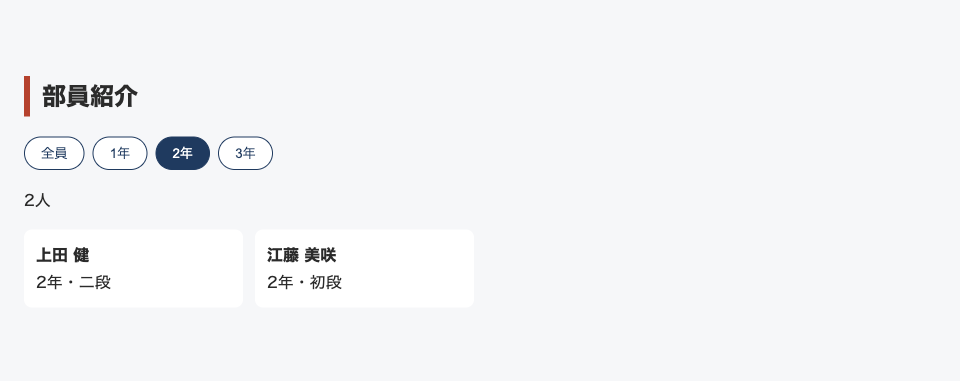
\includegraphics[width=0.47\linewidth]{js-members.png}}\hfill
\fcolorbox{gray!50}{white}{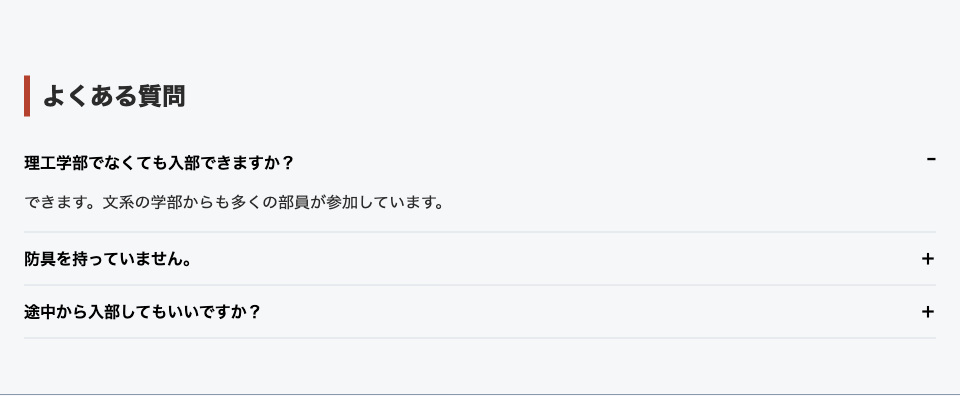
\includegraphics[width=0.47\linewidth]{js-faq.png}}
\end{center}
\figcap{左：学年のボタンで部員を絞り込む　右：質問を押すと答えが開く}

どちらも、\textbf{データ（配列）を用意して、そこから画面を作る}という形で作ります。
これは、第2巻の React でも、第3巻のデータベースでも、本番のサイトでも、ずっと同じ形です。
この章で一番身につけてほしい考え方です。

\section{JavaScript を動かしてみる}

JavaScript は、ブラウザの中で動くプログラミング言語です。
まずはファイルを作らずに、ブラウザの\term{コンソール}で動かしてみます。

\begin{step}{コンソールで計算する}
\sheet{8-1}
ブラウザで \key{F12} を押し、開発者ツールの \menu{Console} タブを開きます。
\code{>} の横に次のように打ち、\key{Enter} を押します。
\begin{terminal}[Console]
> 1 + 2
3
> "面" + "打ち"
'面打ち'
> console.log("稽古開始")
稽古開始
\end{terminal}
\end{step}

\begin{tip}[貼り付けが拒否されたら]
コンソールに初めてコードを貼り付けると、安全のために「allow pasting と入力してください」と表示されることがあります。
これは、知らない人に言われるままコードを貼って乗っ取られる詐欺を防ぐための仕組みです。
この教材のコードは自分で打つので、表示された通りに入力して進めてかまいません。
\end{tip}

\section{変数とデータの型}

\term{変数}は、値に名前をつけて取っておく箱です。

\begin{Piton}[language=code]
const clubName = "理工体剣道部";   // 変えない値は const
let count = 0;                     // あとで変える値は let
count = count + 1;
console.log(clubName, count);      // → 理工体剣道部 1
\end{Piton}

\begin{tip}[const と let の使い分け]
\textbf{基本は \code{const}}、あとで値を入れ直すときだけ \code{let} を使います。
古い資料に出てくる \code{var} は使いません。
\end{tip}

\begin{center}\small
\begin{tabularx}{\linewidth}{l l X}
\toprule
型 & 例 & 説明 \\
\midrule
文字列（string） & \code{"面"}、\code{'小手'} & 文字。\code{"} か \code{'} で囲む \\
数値（number） & \code{4}、\code{18.5} & 計算できる数 \\
真偽値（boolean） & \code{true}、\code{false} & はい／いいえ \\
配列（array） & \code{["面", "小手", "胴"]} & 値の並び。順番がある \\
オブジェクト（object） & \code{\{ name: "上田", grade: 2 \}} & 名前付きの値のまとまり \\
\bottomrule
\end{tabularx}
\end{center}

\begin{caution}["2" と 2 は別物]
\code{"2"} は文字列、\code{2} は数値です。見た目は同じでも、\code{"2" === 2} は \code{false} になります。
画面のボタンから取り出した値はたいてい文字列なので、数値と比べるときは \code{Number("2")} で数値に変換します。
この章の絞り込みで、実際にこの変換が出てきます。
\end{caution}

\section{配列とオブジェクト}

部員1人分の情報は、オブジェクトで表せます。部員全員は、それを並べた配列で表せます。

\begin{Piton}[language=code]
const members = [
  { name: "青木 太郎", grade: 3, dan: "三段", role: "主将" },
  { name: "上田 健",   grade: 2, dan: "二段", role: "" },
];

console.log(members.length);     // → 2（人数）
console.log(members[0].name);    // → 青木 太郎（0 番目の人の名前）
console.log(members[1].grade);   // → 2
\end{Piton}

\begin{why}[配列は 0 番から数える]
配列の最初の要素は \code{[0]}、2番目は \code{[1]} です。最初は戸惑いますが、ほぼすべてのプログラミング言語がこの数え方です。
\end{why}

この「オブジェクトの配列」は、データベースの表とそっくりです。

\begin{center}
\begin{tikzpicture}[font=\sffamily\scriptsize]
  \node[draw=kon,fill=white,align=left,font=\ttfamily\scriptsize,inner sep=6pt] (js) {[\\
  \ \ \{ name: "青木", grade: 3 \},\\
  \ \ \{ name: "上田", grade: 2 \},\\
  ]};
  \node[right=1.8cm of js] (tb) {\begin{tabular}{|l|l|}\hline \rowcolor{kon!15} name & grade\\\hline 青木 & 3\\\hline 上田 & 2\\\hline\end{tabular}};
  \draw[{Stealth}-{Stealth},thick,gray] (js) -- node[above]{同じ形} (tb);
  \node[below=1mm of js] {JavaScript の配列};
  \node[below=1mm of tb] {データベースの表（第3巻）};
\end{tikzpicture}
\end{center}

\section{関数}

\term{関数}は、処理に名前をつけて、何度でも呼び出せるようにしたものです。

\begin{Piton}[language=code]
// 受け取った部員の紹介文を返す関数
function introduce(member) {
  return `${member.grade}年の${member.name}です`;
}

console.log(introduce(members[0]));   // → 3年の青木 太郎です

// 同じ関数を「アロー関数」で書くと、こうなる
const introduce2 = (member) => `${member.grade}年の${member.name}です`;
\end{Piton}

\code{`}（バッククォート）で囲んだ文字列は\term{テンプレートリテラル}といい、\code{\$\{ \}} の中に変数を埋め込めます。
\key{Shift}+\key{@} で入力できます。

\section{条件分岐と繰り返し}

\begin{Piton}[language=code]
// if：条件によって処理を分ける
const member = members[0];
if (member.role === "主将") {
  console.log("主将です");
} else {
  console.log("部員です");
}

// forEach：配列の1人ずつに同じ処理をする
members.forEach((member) => {
  console.log(member.name);
});
\end{Piton}

\begin{tip}[=== を使う]
「等しいか」を調べるときは \code{===}（イコール3つ）を使います。\code{==}（2つ）は型を勝手に変換して比べるので、思わぬ結果になることがあります。
\end{tip}

\section{配列を変換する：filter と map}

この章で一番大事な2つの道具です。

\begin{center}
\begin{tikzpicture}[font=\sffamily\scriptsize,
  item/.style={draw,rounded corners=2pt,minimum width=1.3cm,minimum height=0.55cm,fill=white},
  arr/.style={-{Stealth},thick}]
  \node[font=\sffamily\small\bfseries] at (-1.6,1.2) {filter};
  \foreach \i/\g in {0/3,1/3,2/2,3/2,4/1}{ \node[item] at (\i*1.5,1.2) {\g 年}; }
  \foreach \i/\g in {0/2,1/2}{ \node[item,draw=shu] at (\i*1.5+2.25,0) {\g 年}; }
  \draw[arr,shu] (3,0.85) -- node[right]{\texttt{m => m.grade === 2}} (3,0.35);
  \node[anchor=west] at (6.5,0) {条件に合うものだけ残す};

  \node[font=\sffamily\small\bfseries] at (-1.6,-1.2) {map};
  \foreach \i/\n in {0/青木,1/上田}{ \node[item] at (\i*3+0.75,-1.2) {\n}; }
  \foreach \i/\n in {0/青木,1/上田}{ \node[item,draw=matcha,minimum width=2.6cm,font=\ttfamily\tiny] at (\i*3+0.75,-2.4) {<li>\n</li>}; }
  \draw[arr,matcha] (2.25,-1.55) -- node[right]{1つずつ形を変える} (2.25,-2.05);
  \node[anchor=west] at (6.5,-2.4) {同じ数の、変換後の配列を作る};
\end{tikzpicture}
\end{center}

\begin{Piton}[language=code]
// 2年生だけを取り出す
const second = members.filter((member) => member.grade === 2);

// 名前だけの配列にする
const names = members.map((member) => member.name);   // → ["青木 太郎", "上田 健"]

// HTML の文字列に変換して、つなげる
const html = members.map((member) => `<li>${member.name}</li>`).join("");
\end{Piton}

\section{DOM：JavaScript から HTML を操作する}

ブラウザは、読み込んだ HTML を\term{DOM}という「木」の形で覚えています。
JavaScript はこの木の枝を探して、中身を書き換えたり、クリックを待ち受けたりできます。

\begin{center}\small
\begin{tabularx}{\linewidth}{>{\ttfamily}l X}
\toprule
\normalfont 書き方 & すること \\
\midrule
document.querySelector(".a") & CSS と同じ書き方で、最初に見つかった1つの要素を取ってくる \\
document.querySelectorAll(".a") & 当てはまる要素を全部取ってくる \\
要素.textContent = "..." & 中の文字を書き換える \\
要素.innerHTML = "..." & 中の HTML を書き換える \\
要素.classList.add("x") & class を足す（\code{remove} で外す、\code{toggle} で付け外しを切り替える） \\
要素.addEventListener("click", 関数) & クリックされたら関数を実行する \\
要素.dataset.grade & HTML の \code{data-grade="2"} の値を取り出す \\
\bottomrule
\end{tabularx}
\end{center}

\section{作ってみる}

\begin{step}{HTML に部員紹介の枠を足し、JavaScript を読み込む}
\sheet{8-6}
\code{kendo-top} の \code{index.html} で、「よくある質問」のセクションを、次の2つのセクションに\textbf{置き換えます}。
質問と答えは、HTML に直接書くのをやめ、JavaScript のデータから作ります。
\begin{filebox}{index.html（「よくある質問」のセクションを置き換え）}
\begin{Piton}[language=code]
    <section id="members" class="section">
      <h2>部員紹介</h2>
      <div class="filter">
        <button class="filter-button is-active" data-grade="all">全員</button>
        <button class="filter-button" data-grade="1">1年</button>
        <button class="filter-button" data-grade="2">2年</button>
        <button class="filter-button" data-grade="3">3年</button>
      </div>
      <p class="member-count"></p>
      <ul class="member-list"></ul>
    </section>

    <section id="faq" class="section">
      <h2>よくある質問</h2>
      <div class="faq-list"></div>
    </section>
\end{Piton}
\end{filebox}
さらに、\code{</body>} の直前に次の2行を足します。
\begin{filebox}{index.html（</body> の直前）}
\begin{Piton}[language=code]
  <script src="data.js"></script>
  <script src="script.js"></script>
\end{Piton}
\end{filebox}
\end{step}

\begin{why}[script を body の最後に置く理由]
ブラウザは HTML を上から順に読みます。
\code{<script>} を \code{<head>} に置くと、まだ部員紹介の枠（\code{.member-list}）が作られる前に JavaScript が動いてしまい、
「枠が見つからない」というエラーになります。一番最後に置けば、枠ができあがった後に動きます。
\end{why}

\begin{step}{データのファイルを作る}
\sheet{8-7}
\begin{filebox}{data.js}
\begin{Piton}[language=code]
// 部員のデータ（名前はダミー）
const members = [
  { name: "青木 太郎", grade: 3, dan: "三段", role: "主将" },
  { name: "井上 花子", grade: 3, dan: "二段", role: "女子主将" },
  { name: "上田 健", grade: 2, dan: "二段", role: "" },
  { name: "江藤 美咲", grade: 2, dan: "初段", role: "" },
  { name: "小川 翔", grade: 1, dan: "無", role: "" },
  { name: "加藤 葵", grade: 1, dan: "初段", role: "" },
];

// よくある質問のデータ
const faqs = [
  {
    question: "理工学部でなくても入部できますか？",
    answer: "できます。文系の学部からも多くの部員が参加しています。",
  },
  {
    question: "防具を持っていません。",
    answer: "部の貸し出し用があります。慣れてから自分のものを買う人がほとんどです。",
  },
  {
    question: "途中から入部してもいいですか？",
    answer: "もちろんです。秋から入部する人もいます。",
  },
];
\end{Piton}
\end{filebox}
\textbf{名前はダミーです。}このリポジトリは公開されるので、本物の部員の名前は入れません。
\end{step}

\begin{why}[データと処理を別のファイルに分ける理由]
部員が入れ替わったときに直すのは \code{data.js} だけで済み、処理の \code{script.js} には触らずに済みます。
本番のサイトでは、このデータの置き場所がデータベースになり、管理画面から書き換えられるようになります。
「データと処理を分ける」という考え方が、そのまま本番の仕組みにつながっています。
\end{why}

\begin{step}{よくある質問を作り、クリックで開閉させる}
\sheet{8-8}
\begin{filebox}{script.js}
\begin{Piton}[language=code]
// ===== よくある質問：データから HTML を作り、クリックで開閉する =====
const faqList = document.querySelector(".faq-list");

faqs.forEach((faq) => {
  const item = document.createElement("div");
  item.className = "faq-item";
  item.innerHTML = `
    <button class="faq-question">${faq.question}</button>
    <p class="faq-answer">${faq.answer}</p>
  `;
  faqList.appendChild(item);
});

const questionButtons = document.querySelectorAll(".faq-question");

questionButtons.forEach((button) => {
  button.addEventListener("click", () => {
    const item = button.parentElement;
    item.classList.toggle("is-open");
  });
});

\end{Piton}
\end{filebox}
1行ずつ読むと、次のことをしています。
\begin{enumerate}
  \item \code{.faq-list} の枠を取ってくる
  \item \code{faqs} の1つずつについて、\code{div} を作り、中に質問のボタンと答えの段落を入れて、枠に足す
  \item できあがった質問のボタンを全部取ってくる
  \item それぞれのボタンに「押されたら、親の \code{div} の \code{is-open} を付け外しする」という仕掛けをつける
\end{enumerate}
開いた・閉じたの見た目は、次の STEP の CSS で \code{is-open} が付いているかどうかによって切り替えます。
\textbf{JavaScript は class を付け外しするだけ、見た目は CSS に任せる}、という役割分担です。
\end{step}

\begin{step}{部員紹介を作り、学年で絞り込む}
\sheet{8-9}
\code{script.js} の続きに書きます。
\begin{filebox}{script.js（続き）}
\begin{Piton}[language=code]
// ===== 部員紹介：学年で絞り込む =====
const memberList = document.querySelector(".member-list");
const memberCount = document.querySelector(".member-count");
const filterButtons = document.querySelectorAll(".filter-button");

function renderMembers(grade) {
  // "all" なら全員、それ以外は学年が一致する人だけ残す
  const shown =
    grade === "all"
      ? members
      : members.filter((member) => member.grade === Number(grade));

  memberList.innerHTML = shown
    .map((member) => {
      const role = member.role ? `<span class="role">${member.role}</span>` : "";
      return `<li class="member">${role}<strong>${member.name}</strong><br>${member.grade}年・${member.dan}</li>`;
    })
    .join("");

  memberCount.textContent = `${shown.length}人`;
}

filterButtons.forEach((button) => {
  button.addEventListener("click", () => {
    filterButtons.forEach((b) => b.classList.remove("is-active"));
    button.classList.add("is-active");
    renderMembers(button.dataset.grade);
  });
});

// 最初は全員を表示する
renderMembers("all");
\end{Piton}
\end{filebox}
\code{renderMembers} は「学年を受け取って、その学年の部員で画面を描き直す」関数です。
ボタンが押されるたびに、押されたボタンの \code{data-grade} を渡して呼び出しています。
\code{data-grade} の値は文字列なので、\code{Number(grade)} で数値に変換してから \code{member.grade} と比べています。
\end{step}

\begin{step}{CSS を足す}
\sheet{8-10}
\code{style.css} の \code{/* よくある質問 */} のルール（\code{.faq dt} と \code{.faq dd}）を消して、代わりに次を足します。
\begin{filebox}{style.css}
\begin{Piton}[language=code]
/* 部員紹介 */
.filter {
  display: flex;
  gap: 8px;
}

.filter-button {
  padding: 6px 16px;
  border: 1px solid var(--color-kon);
  border-radius: 999px;
  background-color: white;
  color: var(--color-kon);
  cursor: pointer;
}

.filter-button.is-active {
  background-color: var(--color-kon);
  color: white;
}

.member-list {
  display: grid;
  grid-template-columns: repeat(auto-fill, minmax(180px, 1fr));
  gap: 12px;
  padding: 0;
  list-style: none;
}

.member {
  padding: 12px;
  background-color: white;
  border-radius: 8px;
}

.role {
  display: inline-block;
  margin-right: 6px;
  padding: 0 8px;
  border-radius: 4px;
  background-color: var(--color-shu);
  color: white;
  font-size: 12px;
}

/* よくある質問（開閉） */
.faq-item {
  border-bottom: 1px solid #d9dde3;
}

.faq-question {
  width: 100%;
  padding: 14px 0;
  border: none;
  background: none;
  text-align: left;
  font-size: 16px;
  font-weight: bold;
  cursor: pointer;
}

.faq-question::after {
  content: "＋";
  float: right;
}

.faq-answer {
  display: none;
  margin-top: 0;
}

.faq-item.is-open .faq-answer {
  display: block;
}

.faq-item.is-open .faq-question::after {
  content: "−";
}

\end{Piton}
\end{filebox}
\code{display: grid;} は Flexbox の仲間で、\textbf{縦横のマス目}に並べるときに使います。
\code{repeat(auto-fill, minmax(180px, 1fr))} は「1マス最低 180px で、入るだけ並べる」という意味で、
メディアクエリを書かなくても画面幅に合わせて列の数が自動で変わります。
\end{step}

ブラウザで動きを確かめたら、コミットして push します。

\begin{terminal}[Git Bash]
$ git add index.html data.js script.js style.css
$ git commit -m "feat: よくある質問の開閉と、部員の学年絞り込みを追加"
$ git push
\end{terminal}

\section{エラーの読み方}

JavaScript でつまずいたら、まず開発者ツールの \menu{Console} を見ます。赤い文字がエラーです。

\begin{terminal}[Console]
Uncaught TypeError: Cannot read properties of null (reading 'appendChild')
    at script.js:11:11
\end{terminal}

\begin{center}\small
\begin{tabularx}{\linewidth}{l X}
\toprule
部分 & 読み方 \\
\midrule
\code{TypeError} & エラーの種類。「型が想定と違う」 \\
\code{Cannot read properties of null} & 「\code{null}（何もない）の中身を読もうとした」 \\
\code{(reading 'appendChild')} & 読もうとしたのは \code{appendChild} \\
\code{script.js:11:11} & \textbf{\code{script.js} の11行目}。クリックするとその場所が開く \\
\bottomrule
\end{tabularx}
\end{center}

つまり、「11行目で \code{appendChild} しようとした相手が \code{null}（見つからなかった）」ということです。
よくある原因は、\code{querySelector} に渡したクラス名の打ち間違い（\code{.faq-lsit} など）か、
\code{<script>} を置く場所が早すぎることです。

\begin{center}\small
\begin{tabularx}{\linewidth}{>{\ttfamily\raggedright\arraybackslash}p{5.5cm} X}
\toprule
\normalfont よく出るエラー & よくある原因 \\
\midrule
X is not defined & 変数名の打ち間違い。大文字と小文字も区別される \\
Cannot read properties of null & \code{querySelector} で要素が見つかっていない \\
Cannot read properties of undefined & 配列の範囲外（\code{members[10]}）や、存在しない名前（\code{member.nmae}）を読んだ \\
Unexpected token & かっこやカンマの閉じ忘れ・付けすぎ \\
X is not a function & 関数でないものを \code{()} で呼んだ。名前の打ち間違いが多い \\
\bottomrule
\end{tabularx}
\end{center}

\begin{prompt}[エラーを Claude に聞くとき]
script.js を実行したら、コンソールにこのエラーが出た。\\
（エラーを全文貼る）\\
私は、11行目の faqList が null になっているのが原因だと思っている。この読みが合っているかと、なぜ null になるのかを教えて。直したコードはまだ出さないで。
\end{prompt}

\section{練習問題}
\sheet{8-13〜8-24}

\code{\textasciitilde/dev/js-drill} フォルダを作り、問題ごとにファイル（\code{q01.js} など）を分けて解きます。
1〜9 は、\code{node q01.js} のように Git Bash で実行して結果を確かめられます（Node.js は第3章で入れました）。
10〜12 は HTML と組み合わせるので、ブラウザで確かめます。

\begin{tip}[node で実行する]
\begin{terminal}[Git Bash]
$ cd ~/dev/js-drill
$ node q01.js
\end{terminal}
\code{console.log} で出したものが、そのままターミナルに表示されます。
\end{tip}

\subsection*{基本}

\begin{exercise}[1]{稽古の合計時間}
\toanswer\par
1回の稽古が120分、週に4回、前期が15週あります。前期の稽古時間の合計を「分」で計算して表示してください。
数字はすべて \code{const} の変数に入れ、計算式の中に数字を直接書かないこと。
\end{exercise}

\begin{exercise}[1]{型を当てる}
\toanswer\par
次のそれぞれを \code{console.log} すると何が表示されるか、\textbf{先に予想を書いてから}実行してください。
\begin{Piton}[language=code]
console.log(typeof "4");
console.log(typeof 4);
console.log("4" + 4);
console.log(4 + 4);
console.log("4" === 4);
console.log(Number("4") === 4);
\end{Piton}
\end{exercise}

\begin{exercise}[1]{技の配列}
\toanswer\par
\code{["面", "小手", "胴"]} という配列を作り、次の順に操作して、そのたびに配列全体と長さを表示してください。
(1) 最後に \code{"突き"} を足す　(2) 2番目の要素（\code{"小手"}）だけを表示する　(3) 最後の要素を、長さを使って取り出す
\end{exercise}

\begin{exercise}[1]{自分のプロフィール}
\toanswer\par
自分の名前・学年・学科・好きな技をオブジェクトにまとめ、テンプレートリテラルを使って
「応用化学科2年の柴山です。好きな技は出小手です。」のような文を表示してください。
\end{exercise}

\begin{exercise}[2]{分を「時間と分」に直す関数}
\toanswer\par
分を受け取って、\code{"2時間30分"} のような文字列を返す関数 \code{formatMinutes} を作ってください。
\code{formatMinutes(150)} → \code{"2時間30分"}、\code{formatMinutes(60)} → \code{"1時間0分"}、\code{formatMinutes(45)} → \code{"0時間45分"}。
（ヒント：割り算の余りは \code{\%}、小数の切り捨ては \code{Math.floor}）
余裕があれば、\code{"1時間"}、\code{"45分"} のように0の部分を省略するようにしてください。
\end{exercise}

\begin{exercise}[2]{上級生と下級生}
\toanswer\par
学年を受け取り、1年なら \code{"新入生"}、2年なら \code{"中堅"}、3年以上なら \code{"上級生"}、
それ以外（0 や負の数）なら \code{"学年が正しくありません"} を返す関数を作り、5つの値で試してください。
\end{exercise}

\subsection*{配列の変換}

以下の問題では、本章の \code{data.js} の \code{members} を、ファイルの先頭にコピーして使います。

\begin{exercise}[2]{段位を持っている人}
\toanswer\par
段位が \code{"無"} でない部員だけを取り出し、その人数と名前を表示してください。
\end{exercise}

\begin{exercise}[2]{さん付けの名簿}
\toanswer\par
\code{map} を使って、\code{["青木 太郎さん（3年）", "井上 花子さん（3年）", ...]} という配列を作ってください。
次に、\code{join} を使って、それを改行区切りの1つの文字列にして表示してください。
\end{exercise}

\begin{exercise}[3]{学年ごとの人数}
\toanswer\par
学年ごとの人数を数え、\code{\{ 1: 2, 2: 2, 3: 2 \}} のようなオブジェクトを作って表示してください。
学年が増えても（4年がいても）コードを書き換えずに済むようにすること。
\end{exercise}

\subsection*{画面を動かす}

\begin{exercise}[2]{素振りカウンター}
\toanswer\par
「素振り +1」ボタンと「リセット」ボタン、回数を表示する場所を作ってください。
「+1」を押すたびに回数が1ずつ増え、100回になったら文字の色が朱色に変わるようにします。
（ヒント：色は JavaScript で直接変えず、CSS の class を付け外しする）
\end{exercise}

\begin{exercise}[3]{名前で検索する}
\toanswer\par
本章の部員紹介に、名前の検索欄（\code{<input type="text">}）を足してください。
文字を打つたびに、その文字を名前に含む部員だけが表示されるようにします。
（ヒント：\code{input} イベントと、文字列の \code{includes}）
\end{exercise}

\begin{exercise}[3]{バグを直す}
\toanswer\par
次のコードは、2年生の名前だけを画面に表示するつもりで書かれていますが、\textbf{バグが3つ}あります。
コンソールのエラーを読みながら、すべて直してください。直した理由もそれぞれ1行で書きます。
\begin{filebox}{q12.js}
\begin{Piton}[language=code]
const list = document.querySelector(".member-lsit");
const grade = "2";

const second = members.filter((member) => member.grade === grade);

list.innerHTML = second.map((member) => `<li>${member.nmae}</li>`).join("");
\end{Piton}
\end{filebox}
\end{exercise}


\begin{challenge}{部員紹介に「役職」と「段位」の絞り込みを足す}
\sheet{8-25}
\begin{enumerate}
  \item 学年のボタンの下に、「役職のある人だけ」というチェックボックスを付ける。チェックを入れると、役職（\code{role}）が空でない人だけが表示される
  \item \textbf{学年とチェックボックスは同時に効く}こと（例：3年 ＋ 役職のある人だけ → 主将と女子主将の2人）
  \item 並び順を「学年の高い順、同じ学年なら名前順」にする（ヒント：\code{sort}）
  \item \code{data.js} にダミーの部員を4人足し、表示や人数が正しく変わることを確かめる
\end{enumerate}
\textbf{手を動かす前に}、「\code{renderMembers} のどこを、どう変えれば、2つの条件を同時に効かせられるか」をメモに書いてください。
定例では、そのメモと実際のコードを並べて説明します。
\end{challenge}

\begin{checklist}
\begin{itemize}
  \checkitem \code{const} と \code{let} を使い分けられる
  \checkitem 文字列の \code{"2"} と数値の \code{2} が違うことを説明できる
  \checkitem オブジェクトの配列から、\code{filter} と \code{map} で必要な形を作れる
  \checkitem \code{querySelector} と \code{addEventListener} で、クリックに反応させられる
  \checkitem 「JavaScript は class を付け外しするだけ、見た目は CSS」の役割分担を説明できる
  \checkitem 「データから画面を作る」とはどういうことかを、部員紹介を例に説明できる
  \checkitem コンソールのエラーから、ファイル名と行番号を読み取れる
\end{itemize}
\end{checklist}

\section{第1巻のおわりに}

おつかれさまでした。ここまでで、次のことができるようになりました。

\begin{itemize}
  \item Windows に開発環境を整え、Git と GitHub でコードを管理する
  \item Claude Code に、範囲と完成の条件をはっきりさせて頼み、差分を読んで確かめる
  \item HTML・CSS・JavaScript で、データから画面を作り、インターネットに公開する
\end{itemize}

第2巻では、この章で作った部員紹介と FAQ を、本番のサイトと同じ \textbf{Next.js} で作り直します。
\code{members.filter(...).map(...)} の形が、ほとんどそのまま出てきます。


\appendix
\chapter{コマンド早見表}

\section*{ターミナル（Git Bash）}
\begin{center}\small
\begin{tabularx}{\linewidth}{>{\ttfamily}l X}
\toprule
\normalfont コマンド & すること \\
\midrule
pwd & いま居る場所を表示 \\
ls / ls -a & 中身の一覧／隠しファイルも含めた一覧 \\
cd 場所 / cd .. / cd & 移動／1つ上へ／ホームへ \\
mkdir 名前 & フォルダを作る \\
touch 名前 & 空のファイルを作る \\
cat ファイル & 中身を表示 \\
cp 元 先 / mv 元 先 & コピー／移動・名前変更 \\
rm ファイル & 削除（ゴミ箱に入らない） \\
code . / explorer . & VS Code／エクスプローラーで開く \\
clear & 画面をきれいにする \\
\bottomrule
\end{tabularx}
\end{center}

\section*{Git}
\begin{center}\small
\begin{tabularx}{\linewidth}{>{\ttfamily}l X}
\toprule
\normalfont コマンド & すること \\
\midrule
git init & ここで Git の管理を始める \\
git status & いまの状態を見る（迷ったらこれ） \\
git add ファイル & 変更を準備エリアに入れる \\
git commit -m "メッセージ" & 記録する \\
git push & GitHub に送る（初回は \code{git push -u origin main}） \\
git pull & GitHub の変更を取り込む \\
git clone アドレス & GitHub のリポジトリを丸ごと手元にコピーする \\
git diff & まだ add していない変更を見る \\
git diff --staged & add 済みの変更を見る \\
git log --oneline & 履歴を1行ずつ見る（\code{q} で抜ける） \\
git restore ファイル & add 前の変更を取り消す \\
git restore --staged ファイル & 準備エリアから外す \\
git commit --amend -m "..." & 直前のコミットを直す（push 前だけ） \\
git remote -v & つながっている GitHub のアドレスを見る \\
\bottomrule
\end{tabularx}
\end{center}

\section*{Claude Code}
\begin{center}\small
\begin{tabularx}{\linewidth}{>{\ttfamily}l X}
\toprule
\normalfont 入力 & すること \\
\midrule
claude & 起動（作業したいリポジトリで） \\
/clear & 会話をリセット \\
/compact & 会話を要約して軽くする \\
/status & ログイン状態・使用量 \\
/exit & 終了 \\
\normalfont\key{Esc} / \key{Esc}×2 & 作業を止める／前の発言に戻る \\
\normalfont\key{Shift}+\key{Tab} & モード切り替え（plan mode など） \\
\bottomrule
\end{tabularx}
\end{center}

\section*{Node.js}
\begin{center}\small
\begin{tabularx}{\linewidth}{>{\ttfamily}l X}
\toprule
\normalfont コマンド & すること \\
\midrule
node -v / npm -v & バージョンを確認 \\
node ファイル.js & JavaScript のファイルを実行 \\
npx serve . & いまのフォルダを \code{localhost:3000} で表示 \\
\bottomrule
\end{tabularx}
\end{center}

\chapter{エラー逆引き}

\begin{center}\small
\begin{tabularx}{\linewidth}{>{\ttfamily\raggedright\arraybackslash}p{5.6cm} X l}
\toprule
\normalfont 表示（の一部） & 原因と対処 & 本文 \\
\midrule
command not found & そのコマンドが入っていない／PATH が通っていない。ターミナルを開き直す & 3章 \\
\addlinespace
'irm' is not recognized & PowerShell ではなく CMD で打っている & 3章 \\
\addlinespace
Permission denied (publickey) & SSH 鍵が GitHub に未登録。\code{ssh -T git@github.com} で確認 & 3・5章 \\
\addlinespace
Please tell me who you are & \code{user.name}／\code{user.email} が未設定 & 3章 \\
\addlinespace
not a git repository & Git の管理外のフォルダにいる。\code{pwd} で確認 & 5章 \\
\addlinespace
nothing to commit & 変更がない。保存し忘れていないか & 5章 \\
\addlinespace
! [rejected] (fetch first) & GitHub 側が進んでいる。\code{git pull} してから push & 5章 \\
\addlinespace
このシステムではスクリプトの実行が無効 & PowerShell の安全機能。npm は Git Bash で打つ & 3章 \\
\addlinespace
X is not defined & 変数名の打ち間違い（大文字・小文字も） & 8章 \\
\addlinespace
Cannot read properties of null & \code{querySelector} で要素が見つからない & 8章 \\
\addlinespace
Cannot read properties of undefined & 配列の範囲外や、存在しない名前を読んだ & 8章 \\
\addlinespace
Unexpected token & かっこやカンマの過不足 & 8章 \\
\addlinespace
\normalfont（画像が表示されない） & パスや大文字・小文字の違い。開発者ツールの Network タブで赤い行を探す & 7章 \\
\addlinespace
\normalfont（GitHub Pages が 404） & \code{index.html} の名前と置き場所、Actions タブを確認 & 7章 \\
\bottomrule
\end{tabularx}
\end{center}

\chapter{用語集}

\begin{description}[font=\sffamily\bfseries,leftmargin=0pt,itemsep=3pt]
  \item[API キー] 外部サービスを使うための合言葉。秘密情報なので Git に入れない
  \item[CLI／GUI] 文字で操作する画面／マウスで操作する画面
  \item[CSS] Web ページの見た目を決める言葉
  \item[DOM] ブラウザが HTML を読み込んで作る「木」の形のデータ。JavaScript はこれを操作する
  \item[Flexbox] CSS で要素を横（または縦）に並べる仕組み
  \item[GitHub Pages] GitHub のリポジトリを、そのまま Web サイトとして公開する機能
  \item[HTML] Web ページの中身と構造を書く言葉
  \item[localhost] 自分の PC を指す名前
  \item[Markdown] \code{\#} で見出し、\code{-} で箇条書き、のように記号で書式を付ける書き方
  \item[Node.js] ブラウザの外で JavaScript を動かす道具
  \item[npm／npx] Node.js の道具（パッケージ）を入れる／その場で実行する仕組み
  \item[PATH] コマンドを探しに行くフォルダの一覧
  \item[SSH 鍵] パスワードの代わりに本人確認をするための鍵の組（秘密鍵と公開鍵）
  \item[コミット] Git の記録の単位。「セーブ」に近い
  \item[コンソール] 開発者ツールの中の、JavaScript を打ち込める場所。エラーもここに出る
  \item[差分（diff）] 変更前と変更後の違い
  \item[作業場（ワーキングツリー）] いま編集しているファイルがある場所
  \item[準備エリア（ステージ）] 次のコミットに入れる予定の変更を置く場所
  \item[セレクタ] CSS で「どの要素に」効かせるかを指定する部分
  \item[ターミナル] 文字でコンピュータに命令する画面。この教材では Git Bash
  \item[デプロイ] 作ったものを、インターネットで見られる状態にすること
  \item[ブランチ] 履歴の枝分かれ。第2巻で使う
  \item[フレームワーク] Web アプリを作るための土台一式。Next.js など
  \item[プロンプト] (1) ターミナルの \code{\$} の部分 (2) AI への指示文
  \item[ポート番号] PC の中の「窓口の番号」。\code{localhost:3000} の \code{3000}
  \item[メディアクエリ] 画面の幅などの条件で、CSS を切り替える書き方
  \item[リポジトリ] Git で管理しているフォルダ（とその履歴）
  \item[リモート／origin] GitHub 側のリポジトリ／そのあだ名
  \item[レスポンシブ] 画面の大きさに合わせてレイアウトが変わること
\end{description}

\chapter{練習問題の解答例}

解答は一例です。違う書き方でも、条件を満たしていれば正解です。
自分の答えと違ったら、「どちらが読みやすいか」「なぜその書き方なのか」を考えてみてください。

\section*{第7章}

\subsection*{練習 7.1　見出しの階層}
\begin{Piton}[language=code]
<h1>理工体剣道部の一年</h1>
<h2>春</h2>
<h3>新歓</h3>
<p>新入生の体験稽古を行う。</p>
<h3>早慶戦</h3>
<p>伝統の一戦。</p>
<h2>夏</h2>
<h3>夏合宿</h3>
<p>4泊5日で鍛える。</p>
\end{Piton}
見た目の大きさではなく、\textbf{話の階層}で見出しの番号を選びます。大きさは CSS で変えられます。

\subsection*{練習 7.2　外部リンク}
\begin{Piton}[language=code]
<p>部の Instagram は<a href="https://www.instagram.com/" target="_blank" rel="noopener noreferrer">こちら</a></p>
\end{Piton}
\code{target="\_blank"} で新しいタブが開きます。\code{rel="noopener noreferrer"} は、開いた先のページから元のページを操作されないようにする安全のための設定です。

\subsection*{練習 7.3　画像と代わりの文章}
\begin{Piton}[language=code]
<img src="images/hero.jpg" alt="稽古の後に体育館で撮った部員の集合写真" width="300">
\end{Piton}
\code{alt} は、画像が表示できないときや読み上げソフトで読まれる文章です。「画像」「写真」とだけ書くのではなく、何が写っているかを書きます。

\subsection*{練習 7.4　持ち物リスト}
\begin{Piton}[language=code]
<h3>体験稽古の持ち物</h3>
<ul>
  <li>動きやすい服装</li>
  <li>タオル</li>
  <li>飲み物</li>
  <li>上履き（体育館用）</li>
</ul>
<h3>入部までの流れ</h3>
<ol>
  <li>見学する</li>
  <li>体験稽古に出る</li>
  <li>入部届を出す</li>
</ol>
\end{Piton}
順番に意味がないものは \code{ul}、順番に意味があるものは \code{ol} を使います。

\subsection*{練習 7.5　年間行事の表}
\begin{Piton}[language=code]
<table>
  <thead>
    <tr><th>月</th><th>行事</th><th>区分</th></tr>
  </thead>
  <tbody>
    <tr><td>4月</td><td>新歓・体験稽古</td><td>イベント</td></tr>
    <tr><td>6月</td><td>早慶戦</td><td>試合</td></tr>
    <tr><td>8月</td><td>夏合宿</td><td>合宿</td></tr>
    <tr><td>3月</td><td>春合宿</td><td>合宿</td></tr>
  </tbody>
</table>
\end{Piton}

\subsection*{練習 7.6　間違い探し}
\begin{enumerate}
  \item \code{<h2>稽古について<h2>}：終了タグの \code{/} がない → \code{</h2>}
  \item \code{<strong>週4回</p></strong>}：閉じる順番が逆。後に開いたものから先に閉じる → \code{<strong>週4回</strong></p>}
  \item \code{<ul>} の中に \code{<p>}：\code{ul} の直下には \code{li} しか置けない → \code{<li>火曜日</li>}
  \item \code{<img>} に \code{alt} がない → \code{alt="..."} を付ける
\end{enumerate}
ブラウザは間違った HTML でもなんとか表示しようとするので、見た目では気づきにくいのが厄介なところです。

\subsection*{練習 7.7　問い合わせフォーム}
\begin{Piton}[language=code]
<form>
  <label for="name">名前</label>
  <input type="text" id="name" name="name" required>

  <label for="email">メールアドレス</label>
  <input type="email" id="email" name="email" required>

  <label for="message">問い合わせ内容</label>
  <textarea id="message" name="message" rows="5"></textarea>

  <button type="submit">送信する</button>
</form>
\end{Piton}
\code{label} の \code{for} と \code{input} の \code{id} を同じ値にすると、ラベルを押したときに入力欄が選ばれます。
\code{type="email"} でメールの形のチェック、\code{required} で空欄のチェックをブラウザがしてくれます。
ただし、これは\textbf{ブラウザ側のチェックにすぎず、悪意のある人は簡単にすり抜けられます}。
第4巻で、サーバー側でもチェックする理由を学びます。

\subsection*{練習 7.8　サイトの色を一気に変える}
\begin{Piton}[language=code]
:root {
  --color-kon: #1e4d3a;
  --color-shu: #b8860b;
  --color-bg: #f6f7f9;
  --color-text: #2b2b2b;
}
\end{Piton}
CSS 変数を使うと、\textbf{色を変えたいときに直す場所が1か所で済み、直し忘れが起きません}。

\subsection*{練習 7.9　セレクタはどれに効く？}
赤くなるのは「新歓稽古を行います。」と「雨天でも実施します。」の2つです。
\begin{itemize}
  \item \code{.news p}：\code{.news} の中の \code{p} すべて。\code{class="important"} が付いていても \code{p} なので当てはまる
  \item \code{\#top}：\code{id="top"} の要素はないので、どこにも効かない
  \item \code{h3}：\code{h3} はないので、どこにも効かない
  \item \code{section} の外の \code{p.important} は、\code{.news} の中ではないので赤くならない
\end{itemize}

\subsection*{練習 7.10　箱の幅を計算する}
\begin{enumerate}
  \item 指定なし：中身 300 ＋ 左右の padding 20×2 ＋ 左右の枠線 2×2 ＝ \textbf{344px}
  \item \code{border-box}：padding と枠線が 300px の中に含まれるので \textbf{300px}
\end{enumerate}
どちらの場合も、margin（10px）は箱の外側の余白なので、横幅には含みません（となりとの間隔になります）。
開発者ツールの \menu{Computed} タブに、この箱の図と数字が表示されます。

\subsection*{練習 7.11　ボタンに反応をつける}
\begin{Piton}[language=code]
.button {
  /* もとの指定はそのまま。この1行を足す */
  transition: background-color 0.2s;
}

.button:hover {
  background-color: #8f3424;
}
\end{Piton}

\subsection*{練習 7.12　フッターを3列にする}
\begin{Piton}[language=code]
<footer class="site-footer">
  <div class="footer-inner">
    <div>
      <p class="footer-title">理工体剣道部</p>
      <p>慶應義塾大学 理工学部體育會剣道部</p>
    </div>
    <div>
      <p class="footer-title">稽古場所</p>
      <p>矢上キャンパス 体育館</p>
    </div>
    <div>
      <p class="footer-title">SNS</p>
      <p><a href="https://www.instagram.com/">Instagram</a></p>
    </div>
  </div>
</footer>
\end{Piton}
\begin{Piton}[language=code]
.footer-inner {
  display: flex;
  justify-content: space-between;
  max-width: 960px;
  margin: 0 auto;
  text-align: left;
}

.footer-title {
  font-weight: bold;
}

.site-footer a {
  color: white;
}

@media (max-width: 640px) {
  .footer-inner {
    flex-direction: column;
  }
}
\end{Piton}

\subsection*{練習 7.13　どちらの CSS が勝つ？}
\textbf{緑}になります。
同じ要素に複数のルールが当たったとき、より「具体的な」セレクタが勝ちます。これを\term{詳細度}といいます。
おおまかには「id の数 → class の数 → タグの数」の順に比べます。
\begin{center}\small
\begin{tabular}{lccc}\toprule
セレクタ & id & class & タグ \\\midrule
\code{\#main-title} & 1 & 0 & 0 \\
\code{h2.title} & 0 & 1 & 1 \\
\code{.title} & 0 & 1 & 0 \\\bottomrule
\end{tabular}
\end{center}
\code{.title} を勝たせるには、それ以上に具体的にします。たとえば \code{\#main-title.title \{ color: red; \}} は id 1・class 1 なので勝ちます。
ただし、詳細度の競争を始めるとどんどん読みにくくなるので、\textbf{そもそも id で見た目を付けない}のが一番の対策です。

\subsection*{練習 7.14　タブレットでは2列にする}
\begin{Piton}[language=code]
.cards {
  display: flex;
  flex-wrap: wrap;
  gap: 16px;
}

.card {
  /* 3枚並べる：全体から隙間2つ分を引いて3等分 */
  flex: 0 0 calc((100% - 32px) / 3);
}

@media (max-width: 960px) {
  .card {
    flex-basis: calc((100% - 16px) / 2);
  }
}

@media (max-width: 640px) {
  .card {
    flex-basis: 100%;
  }
}
\end{Piton}
もとの \code{@media (max-width: 640px)} の中の \code{.cards \{ flex-direction: column; \}} は、消しても同じ見た目になります。

\subsection*{練習 7.15　開発者ツールで原因を探す}
\begin{enumerate}
  \item \menu{Elements} で \code{h2} を選ぶと、右の \menu{Styles} に \code{.section h2} のルールが出ます。右上に \code{style.css:行番号} と表示され、そこに \code{border-left: 6px solid var(--color-shu);} があります
  \item \code{6px} をクリックして \code{12px} に変えると、線が太くなります
  \item 再読み込みすると 6px に戻ります。開発者ツールでの変更は、ファイルには保存されません
\end{enumerate}

\subsection*{練習 7.16　見本を再現する}
\begin{Piton}[language=code]
<section class="section">
  <h2>数字で見る剣道部</h2>
  <div class="stats">
    <div class="stat"><p class="stat-number">52</p><p class="stat-label">部員数</p></div>
    <div class="stat"><p class="stat-number">4</p><p class="stat-label">週の稽古回数</p></div>
    <div class="stat"><p class="stat-number">2</p><p class="stat-label">年間の合宿</p></div>
    <div class="stat"><p class="stat-number">70</p><p class="stat-label">初心者・リバ剣の割合（%）</p></div>
  </div>
</section>
\end{Piton}
\begin{Piton}[language=code]
.stats {
  display: grid;
  grid-template-columns: repeat(4, 1fr);
  gap: 12px;
}

.stat {
  padding: 16px;
  text-align: center;
  background-color: white;
  border-radius: 8px;
}

.stat-number {
  margin: 0;
  font-size: 40px;
  font-weight: bold;
  color: var(--color-shu);
}

.stat-label {
  margin: 0;
  font-size: 12px;
  color: #888;
}

@media (max-width: 640px) {
  .stats {
    grid-template-columns: repeat(2, 1fr);
  }
}
\end{Piton}

\section*{第8章}

\subsection*{練習 8.1　稽古の合計時間}
\begin{Piton}[language=code]
const minutesPerPractice = 120;
const practicesPerWeek = 4;
const weeks = 15;

const total = minutesPerPractice * practicesPerWeek * weeks;
console.log(`前期の稽古時間は ${total} 分`);   // → 7200 分
\end{Piton}
数字に名前をつけておくと、あとで読んだときに「120 って何だっけ」とならずに済みます。

\subsection*{練習 8.2　型を当てる}
\begin{Piton}[language=code]
typeof "4"          // "string"
typeof 4            // "number"
"4" + 4             // "44"   文字列があると、+ は「つなげる」になる
4 + 4               // 8
"4" === 4           // false  型が違う
Number("4") === 4   // true
\end{Piton}

\subsection*{練習 8.3　技の配列}
\begin{Piton}[language=code]
const waza = ["面", "小手", "胴"];

waza.push("突き");
console.log(waza, waza.length);          // → ["面","小手","胴","突き"] 4

console.log(waza[1]);                    // → 小手

console.log(waza[waza.length - 1]);      // → 突き
\end{Piton}
\code{const} で作った配列でも、\code{push} で中身を足すことはできます。\code{const} が禁止しているのは「箱ごと入れ替えること」だけです。

\subsection*{練習 8.4　自分のプロフィール}
\begin{Piton}[language=code]
const me = {
  name: "柴山",
  grade: 2,
  department: "応用化学科",
  favoriteWaza: "出小手",
};

console.log(`${me.department}${me.grade}年の${me.name}です。好きな技は${me.favoriteWaza}です。`);
\end{Piton}

\subsection*{練習 8.5　分を「時間と分」に直す関数}
\begin{Piton}[language=code]
function formatMinutes(totalMinutes) {
  const hours = Math.floor(totalMinutes / 60);
  const minutes = totalMinutes % 60;
  return `${hours}時間${minutes}分`;
}

// 0 の部分を省略する版
function formatMinutesShort(totalMinutes) {
  const hours = Math.floor(totalMinutes / 60);
  const minutes = totalMinutes % 60;
  if (hours === 0) return `${minutes}分`;
  if (minutes === 0) return `${hours}時間`;
  return `${hours}時間${minutes}分`;
}

console.log(formatMinutes(150));        // → 2時間30分
console.log(formatMinutesShort(60));    // → 1時間
console.log(formatMinutesShort(45));    // → 45分
\end{Piton}

\subsection*{練習 8.6　上級生と下級生}
\begin{Piton}[language=code]
function gradeLabel(grade) {
  if (grade === 1) {
    return "新入生";
  } else if (grade === 2) {
    return "中堅";
  } else if (grade >= 3) {
    return "上級生";
  } else {
    return "学年が正しくありません";
  }
}

[1, 2, 3, 4, 0].forEach((g) => console.log(g, gradeLabel(g)));
\end{Piton}

\subsection*{練習 8.7　段位を持っている人}
\begin{Piton}[language=code]
const withDan = members.filter((member) => member.dan !== "無");
console.log(withDan.length);
withDan.forEach((member) => console.log(member.name));
\end{Piton}

\subsection*{練習 8.8　さん付けの名簿}
\begin{Piton}[language=code]
const roster = members.map((member) => `${member.name}さん（${member.grade}年）`);
console.log(roster);
console.log(roster.join("\n"));
\end{Piton}
\code{\textbackslash n} は改行を表す特別な文字です。

\subsection*{練習 8.9　学年ごとの人数}
\begin{Piton}[language=code]
const counts = {};

members.forEach((member) => {
  // まだその学年の数を数えていなければ 0 から始める
  if (counts[member.grade] === undefined) {
    counts[member.grade] = 0;
  }
  counts[member.grade] = counts[member.grade] + 1;
});

console.log(counts);   // → { '1': 2, '2': 2, '3': 2 }
\end{Piton}
オブジェクトの名前（キー）を、\code{counts[member.grade]} のように変数で指定しているのがポイントです。
この「グループごとに数える」処理は、第3巻の SQL の \code{GROUP BY} でもう一度出てきます。

\subsection*{練習 8.10　素振りカウンター}
\begin{Piton}[language=code]
<p class="count">0</p>
<button class="plus">素振り +1</button>
<button class="reset">リセット</button>

<style>
  .count.is-goal { color: #b5422e; font-weight: bold; }
</style>

<script>
  const GOAL = 100;
  const countText = document.querySelector(".count");
  let count = 0;

  function update() {
    countText.textContent = count;
    if (count >= GOAL) {
      countText.classList.add("is-goal");
    } else {
      countText.classList.remove("is-goal");
    }
  }

  document.querySelector(".plus").addEventListener("click", () => {
    count = count + 1;
    update();
  });

  document.querySelector(".reset").addEventListener("click", () => {
    count = 0;
    update();
  });
</script>
\end{Piton}
\code{count} はあとで値を入れ直すので \code{let}、目標の 100 は変えないので \code{const} です。

\subsection*{練習 8.11　名前で検索する}
\begin{Piton}[language=code]
<!-- index.html：部員紹介の .filter の下に足す -->
<input type="text" class="member-search" placeholder="名前で検索">
\end{Piton}
\begin{Piton}[language=code]
// script.js：一番最後に足す
const searchInput = document.querySelector(".member-search");

searchInput.addEventListener("input", () => {
  const keyword = searchInput.value.trim();
  const shown = members.filter((member) => member.name.includes(keyword));

  memberList.innerHTML = shown
    .map((member) => `<li class="member"><strong>${member.name}</strong><br>${member.grade}年・${member.dan}</li>`)
    .join("");
  memberCount.textContent = `${shown.length}人`;
});
\end{Piton}
この解答では、学年のボタンと検索欄が別々に動きます（検索すると学年の絞り込みが無視される）。
両方を同時に効かせる方法は、本章の腕だめしで考えます。

\subsection*{練習 8.12　バグを直す}
\begin{Piton}[language=code]
const list = document.querySelector(".member-list");   // ① lsit → list

const grade = 2;                                       // ② 文字列 "2" ではなく数値 2

const second = members.filter((member) => member.grade === grade);

list.innerHTML = second.map((member) => `<li>${member.name}</li>`).join("");   // ③ nmae → name
\end{Piton}
\begin{enumerate}
  \item クラス名の打ち間違いで要素が見つからず、\code{list} が \code{null} になっていた（\code{Cannot read properties of null}）
  \item \code{member.grade} は数値なので、文字列の \code{"2"} とは \code{===} で一致せず、誰も残らなかった（エラーは出ないので一番気づきにくい）
  \item 存在しない \code{nmae} を読んだため、名前が \code{undefined} と表示されていた
\end{enumerate}
②のように、\textbf{エラーが出ないのに結果がおかしい}バグが一番やっかいです。
「何人残ったか」を \code{console.log(second.length)} で確かめるなど、途中の値を表示して追いかけるのが基本です。


\end{document}
